
 

\chapter{The Real Numbers}\label{ch1}

 \section{Logic, Sets and Functions}
 
In this section, we give a brief review of propositional logic, sets and functions.  It is assumed that students have taken an introductory course which covers these topics, such as a course in discrete mathematics \cite{Rosen}. 

\begin{definition}{Proposition} 
A {\bf proposition}, usually denoted by $p$, is a declarative sentence that is either true or false, but not both.
\end{definition}

\begin{definition}{Negation of a Proposition}
 If $p$ is a proposition, $\neg p$ is the {\bf negation} of $p$. The proposition $p$ is true if and only if the negation $\neg p$ is false.
\end{definition}

From two propositions $p$ and $q$, we can apply logical operators and   obtain a compound proposition. 

\begin{definition}{Conjunction of   Propositions}
 If $p$ and $q$ are propositions, $p\wedge q$ is the {\bf conjunction} of $p$ and $q$, read as "$p$ and $q$". The proposition $p\wedge q$ is true if and only if both $p$ and $q$ are true.
\end{definition}

\begin{definition}{Disjunction of   Propositions}
 If $p$ and $q$ are propositions, $p\vee q$ is the {\bf disjunction} of $p$ and $q$, read as "$p$ or $q$". The proposition $p\vee q$ is true if and only if either $p$ is true or $q$ is true.
\end{definition}

\begin{definition}{Implication of   Propositions}
 If $p$ and $q$ are propositions, the proposition $p\to q$ is read as "$p$ {\bf implies} $q$". It is false if and only if $p$ is true but $q$ is false.
\end{definition}

$p\to q$ can also be read as "if $p$ then $q$ or "$p$ only if $q$". In mathematics, we usually write $p\implies q$ instead of $p\to q$. 

\begin{definition}{Double Implication}
 If $p$ and $q$ are propositions, the proposition $p\longleftrightarrow q$ is read as "$p$ {\bf if and only if} $q$". It is the conjunction of $p\to q$ and $q\to p$. Hence, it is true if and only if both $p$ and $q$ are true, or both $p$ and $q$ are false.
\end{definition}

The stament ``$p$ if and only if $q$'' is often expressed as $p\iff q$.

Two compound propositions $p$ and $q$ are said to be logically equivalent, denoted by $p\equiv q$, provided that $p$ is true if and only if $q$ is true. 


Logical equivalences are important for working with mathematical proofs. Some equivalences such as commutative law, associative law, distributive law are obvious. Other important equivalences are listed in the theorem below.
\begin{theorem}{Logical Equivalences}

Let $p$, $q$, $r$ be propositions. 
\begin{enumerate}[1.]
\item $p\to q \;\equiv \;\neg p\vee q$
\item De Morgan's Law
\begin{enumerate}[(i)]
\item $\neg(p\vee q)\;\equiv\;\neg p\,\wedge\,\neg q$
\item $\neg(p\wedge q)\;\equiv\;\neg p\,\vee\,\neg q$
\end{enumerate}

\end{enumerate}
\end{theorem}

A very important equivalence is the equivalence of an implication with its contrapositive.
\begin{theorem}{Contraposition}
If $p$ and $q$ are propositions, $p\to q$ is equivalent to $\neg q\to\neg p$.
\end{theorem}

In mathematics, we are often dealing with statements that depend on variables. Quantifiers are used to specify the extent to which such a statement is true. Two commonly used quantifiers are "for all" ($\forall$) and "there exists" ($\exists$). 

For negation of statements with quantifiers, we have the following generalized De Morgan's law.

\begin{theorem}{Generalized De Morgan's Law}
\begin{enumerate}[1.]
\item $\neg\left(\forall x\;P(x)\right)\;\equiv\;\exists x\;\neg P(x)$
\item $\neg\left(\exists x\;P(x)\right)\;\equiv\;\forall x\;\neg P(x)$
\end{enumerate}
\end{theorem}

For nested quantifiers, the ordering is important if different types of quantifiers are involved. For example, the statement
\[\forall x\;\exists y\; \;x+y=0\] is not equivalent to the statement
\[\exists y\;\forall x\;\;x+y=0.\]When the domains for $x$ and $y$ are both the set of real numbers, the first statement is true, while the second statement is false.


 
For a set $A$, we use the notation $x\in A$ to denote $x$ is an element of the set $A$; and the notation $x\notin A$ to denote $x$ is not an element of $A$.

\begin{definition}{Equal Sets}
Two sets $A$ and $B$ are equal if they have the same elements. In logical expression, $A=B$ if and only if
\[x\in A\iff x\in B.\]
\end{definition}

\begin{definition}
{Subset}
If $A$ and $B$ are sets, we say that $A$ is a {\bf subset} of $B$,  denoted by $A\subset B$, if every element of $A$ is an element of $B$. In logical expression, $A\subset B$ means that
\[x\in A\implies x\in B.\]
\end{definition}

When $A$ is a subset of $B$, we will also say that  $A$ is contained in $B$, or $B$ contains $A$.


We say that $A$ is a {\bf proper subset} of $B$ if $A$ is a subset of $B$ and $A\neq B$. 
In some textbooks,  the symbol "$\subseteq$" is used to denote subset, and the symbol "$\subset$" is reserved for proper subset. In this book, we will not make such a distinction. Whenever we write $A\subset B$, it means $A$ is a subset of $B$, not necessary a proper subset.

There are   operations that can be defined on sets, such as union, intersection, difference and complement. 

\begin{definition}
{Union of Sets}
If $A$ and $B$ are sets, the {\bf union} of $A$ and $B$ is the set $A\cup B$ which contains all elements that are either in $A$ or in $B$. In logical expression,
\[x\in A\cup B\iff (x\in A)\;\vee\;(x\in B).\]
\end{definition}

\begin{definition}
{Intersection of Sets}
If $A$ and $B$ are sets, the {\bf intersection} of $A$ and $B$ is the set $A\cap B$ which contains all elements that are  in both $A$ and  $B$. In logical expression,
\[x\in A\cap B\iff (x\in A)\;\wedge\;(x\in B).\]
\end{definition}

\begin{definition}
{Difference of Sets}
If $A$ and $B$ are sets, the difference of $A$ and $B$ is the set $A\setminus B$  which contains all elements that are  in  $A$ and not in  $B$. In logical expression,
\[x\in A\setminus B\iff (x\in A)\;\wedge\;(x\notin B).\]
\end{definition}

\begin{definition}
{Complement of a Set}
If $A$ is a set that is contained in a universal set $U$, the {\bf complement} of $A$ in $U$ is the set $A^C$ which contains all elements that are in $U$ but not in $A$. In logical expression,
\[x\in A^C\iff (x\in U)\;\wedge\;(x\notin A).\]
\end{definition}

Since a universal set can vary from context to context, we will usually avoid using the notation $A^C$ and use $U\setminus A$ instead for the complement of $A$ in $U$. The advantage of using the notation $A^C$ is that De Morgan's law takes a more succint form.

\begin{proposition}{De Morgan's Law for Sets}

If $A$ and $B$ are sets in a universal set $U$, and $A^C$ and $B^C$ are their complements in $U$, then
\begin{enumerate}[1.]
\item
$(A\cup B)^C=A^C\cap B^C$
\item $(A\cap B)^C=A^C\cup B^C$
\end{enumerate}
\end{proposition}

\begin{definition}{Functions}
When $A$ and $B$ are sets, a {\bf function} $f$ from $A$ to $B$, denoted by $f:A\rightarrow B$, is a correspondence that assigns every element of $A$ a unique element in $B$. If $a$ is in $A$, the {\bf image} of $a$ under the function $f$ is denoted by $f(a)$, and it is an element of $B$.

$A$ is called the {\bf domain} of $f$, and $B$ is called the {\bf codomain} of $f$.
\end{definition}
\begin{definition}
{Image of a Set}
If $f:A\to B$ is a function and $C$ is a subset of $A$, the image of $C$ under $f$ is the set 
\[f(C)=\left\{f(c)\,|\,c\in C\right\}.\]
$f(A)$ is called the range of $f$.

\end{definition} 


\begin{definition}
{Preimage of a Set}
If $f:A\to B$ is a function and $D$ is a subset of $B$, the preimage of $D$ under $f$ is the set 
\[f^{-1}(D)=\left\{a\in A\,|\,f(a)\in D\right\}.\]
 
\end{definition} 
Notice that $f^{-1}(D)$ is a notation, it does not mean that the function $f$ has an inverse.

Next, we turn to discuss injectivity and surjectivity of functions.
\begin{definition}{Injection}
We say that a function $f:A\to B$ is an {\bf injection}, or the function $f:A\rightarrow B$ is {\bf injective}, or the function $f:A\to B$ is {\bf one-to-one}, if no pair of distinct elements of $A$ are mapped to the same element of $B$.
Namely,
\[a_1\neq a_2 \implies f(a_1)\neq f(a_2).\]

\end{definition}

Using contrapositive, a function is injective provided that
\[f(a_1)=f(a_2)\implies a_1=a_2.\]


\begin{definition}{Surjection}
We say that a function $f:A\to B$ is a {\bf surjection}, or the function $f:A\rightarrow B$ is {\bf surjective}, or the function $f:A\to B$ is {\bf onto}, if every element of $B$ is the image of some element in $A$.
Namely,
\[\forall b\in B, \exists a\in A, f(a)=b.\]
Equivalently, $f:A\to B$ is surjective if the range of $f$ is $B$. Namely, $f(A)=B$.

\end{definition}

\begin{definition}{Bijection}
We say that a function $f:A\to B$ is a {\bf bijection}, or the function $f:A\rightarrow B$ is bijective, if it is both injective and surjective.

A bijection is also called a  {\bf one-to-one correspondence}.

\end{definition}

Finally, we would like to make a remark about some notations. If $f:A\rightarrow B$ is a function with domain $A$, and $C$ is a subset of $A$, the restriction of $f$ to $C$ is the function $f|_C:C\rightarrow B$ defined by $f|_C(c)=f(c)$ for all $c\in C$. When no confusion arises, we will often denote this function simply as $f:C\rightarrow B$.
\vp
\section{The Set of Real Numbers and Its Subsets}\label{sec1.2}
In this section, we introduce the set of real numbers using an intuitive approach. 

\begin{definition}{Natural Numbers}
The set of {\bf natural numbers} $\mathbb{N}$ is the set that contains the counting numbers,    1, 2, 3 $\ldots$, which are also called positive integers. 
\end{definition}

$\mathbb{N}$ is an inductive set. The number 1 is the smallest element of this set. If $n$ is a natural number, then $n+1$ is also a natural number.  

The number 0 corresponds to nothing. 

For every positive integer $n$, $-n$ is a number which   produces 0 when adds to $n$. This number $-n$ is called the negative of $n$, or the additive inverse of $n$.

$-1$, $-2$, $-3$, $\ldots$, are called negative integers.

\begin{definition}{Integers}
The set of {\bf integers} $\mathbb{Z}$ is the set that contains all positive integers, negative integers and 0.
\end{definition}

We will also use the notation $\mathbb{Z}^+$ to denote the set of positive integers. 

\begin{definition}{Rational Numbers}
 The set of {\bf rational numbers} $\mathbb{Q}$ is the set defined as
\[\mathbb{Q}=\left\{\left.\frac{m}{n}\,\right|\,m,n\in\mathbb{Z}, n\neq 0\right\}.\]
\end{definition}

Each rational number is a quotient of two integers, where the denominator is nonzero. The set of integers $\mathbb{Z}$ is a subset of the set of rational numbers $\mathbb{Q}$.

Every rational number $m/n$ has a decimal expansion. For example, 
\[-\frac{23}{4}=-5.75,\]
\[\frac{27}{7}=3.857142857142\ldots=3.\dot{8}5714\dot{2}.\]
The decimal expansion of a rational number is either finite or periodic.

\begin{definition}{Real Numbers}
The set of {\bf real numbers} $\mathbb{R}$ is intuitively defined to be the set that contains all decimal numbers, which is not necessary periodic. 
\end{definition}

The set of real numbers contains the set of rational numbers $\mathbb{Q}$ as a subset. If a real number is not a rational number, we call it an {\bf irrational number}. The set of irrational numbers is $\mathbb{R}\setminus\mathbb{Q}$.

 

It has been long known that there are real numbers that are not   rational numbers. The best example is the number $\sqrt{2}$, which appears as the length of the diagonal of a unit square (see Figure \ref{figure1}).

\begin{figure}[ht]
\centering
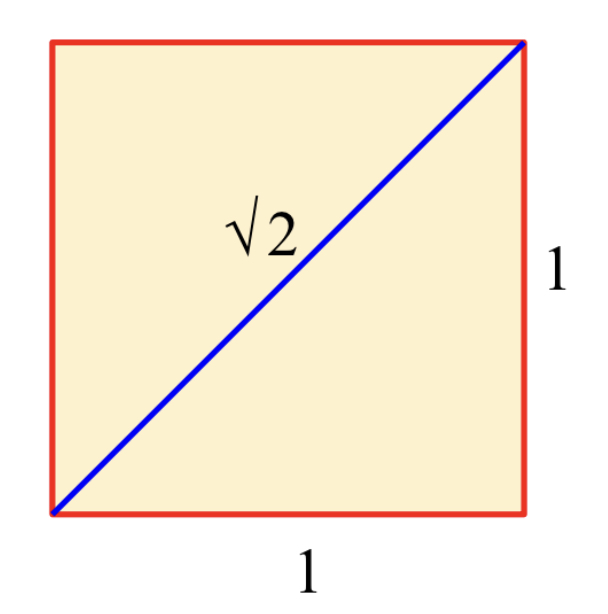
\includegraphics[scale=0.2]{Picture1.png}

\caption{The number $\sqrt{2}$.}\label{figure1}
\end{figure}




The   addition and multiplication operations defined on the set of natural numbers can be extended to the set of real numbers consistently. 

If $a$ and $b$ are  real numbers, $a+b$ is the addition of  $a$ and $b$, and $ab$ is the multiplication of $a$ and $b$.

If $a$ and $b$ are positive real numbers, $a+b$ and $ab$ are also positive real numbers.



The set of real numbers with the addition and multuplication operations is a field, which you will learn in abstract algebra. These operations satisfy the following properties.


 
 \begin{highlight}{Properties of Real Numbers}

 
         \begin{enumerate} [1.]
\item
\textbf{Commutativity of Addition}
\[a+b=b+a\]
\item \textbf{Associativity of Addition}
\[(a+b)+c=a+(b+c)\]
\item\textbf{Additive Identity }
\[a+0=0+a=a\]
0 is called the additive identity.
\item\textbf{Additive Inverse}
\\For every real number $a$, the negative of $a$, denoted by $-a$, satisfies
\[a+(-a)=(-a)+a=0\]

\item
\textbf{Commutativity of Multiplication}
\[ab=ba\]
\item \textbf{Associativity of Multiplication}
\[(ab)c=a(bc)\]

\item\textbf{Multiplicative Identity }
\[a\cdot 1=1\cdot a=a\]
1 is called the multiplicative identity.
\item\textbf{Multiplicative Inverse}
\\For every nonzero real number $a$, the reciprocal of $a$, denoted by $1/a$, satisfies
\[a\cdot \frac{1}{a}=\frac{1}{a}\cdot a=1\]
\item \textbf{Distributivity}
\[a(b+c)=ab+ac\]
\end{enumerate}
 \end{highlight}



\vfill\pagebreak
 
The set of complex numbers $\mathbb{C}$ is the set that contains all numbers of the form $a+ib$, where $a$ and $b$ are real numbers, and $i$ is the purely imaginary number such that $i^2=-1$. It contains the set of real numbers $\mathbb{R}$ as a subset. Addition and multiplication can be extended to the set of complex numbers. These two operations on complex numbers also satisfy all the properties listed above. Nevertheless, we shall focus on the set of real numbers in this course.


There are special subsets of real numbers which are called {\bf intervals}.  There are nine types of intervals, four types are finite, five types are semi-infinite or infinite.  Their definitions are as follows. 

\begin{highlight}{Finite Intervals}

\begin{enumerate}
\item[1.] $(a,b)=\di\left\{x\in\mathbb{R}\,|\, a<x<b\right\}$
\item[2.] $[a,b)=\di\left\{x\in\mathbb{R}\,|\, a\leq x<b\right\}$
\item[3.] $(a,b]=\di\left\{x\in\mathbb{R}\,|\, a<x\leq b\right\}$
\item[4.] $[a,b]=\di\left\{x\in\mathbb{R}\,|\, a\leq x \leq b\right\}$
\end{enumerate}
\end{highlight}

For the intervals $(a, b)$, $[a, b)$, $(a, b]$, $[a, b]$, the points $a$ and $b$ are the {\bf end points} of the interval, while any point $x$ with $a<x<b$ is an {\bf interior point}.

\begin{highlight}{Semi-Infinite or Infinite Intervals}
\begin{enumerate}
\item[5.] $(a,\infty)=\di\left\{x\in\mathbb{R}\,|\, x>a\right\}$
\item[6.] $[a,\infty)=\di\left\{x\in\mathbb{R}\,|\, x\geq a\right\}$
\item[7.] $(-\infty, a)=\di\left\{x\in\mathbb{R}\,|\, x<a\right\}$
\item[8.] $(-\infty, a]=\di\left\{x\in\mathbb{R}\,|\, x\leq a\right\}$
\item[9.] $(-\infty, \infty)=\mathbb{R}$.
\end{enumerate}
\end{highlight}

  For  the intervals $(a, \infty)$, $[a, \infty)$, $(-\infty, a)$ and $(-\infty, a]$, $a$ is the {\bf end point} of the interval, while any other points in the interval besides $a$ is an {\bf interior point}.

The set of natural numbers is a well-ordered set. Every nonempty subset of positive integers has a smallest element.  This statement is equivalent to the principle of mathematical induction, which is one of the  important strategies in proving mathematical statements.

\begin{proposition}{Principle of Mathematical Induction}
Let $P(n)$ be a sequence of statements that are indexed by the set of positive integers $\mathbb{Z}^+$. Assume that the following two assertions are true.
\begin{enumerate}[1.]
\item The statement $P(1)$ is true.
\item For every positive integer $n$, if the statement $P(n)$ is true, the statement $P(n+1)$ is also true.
\end{enumerate}Then we can conclude that for all positive integers $n$, the statement $P(n)$ is true.

\end{proposition}


Before ending this section, let us discuss the absolute value and some useful inequalities.
\begin{definition}{Absolute Value}
Given a real number $x$, the {\bf absolute value} of $x$, denoted by $|x|$, is defined to be the nonnegative number
\[|x|=\begin{cases}x,\quad &\text{if}\;x\geq 0,\\-x,\quad &\text{if}\;x<0.\end{cases}\]
In particular, $|-x|=|x|$.
\end{definition}

For example, $|2.7|=2.7$, $|-2.7|=2.7$. 

The absolute value  $|x|$ can be interpreted as the distance between the number $x$ and the number $0$ on the number line. For any two real numbers $x$ and $y$, $|x-y|$ is the distance between $x$ and $y$. Hence, the  absolute value can be used to express an interval.
\begin{highlight}{Intervals Defined by Absolute Values}
Let $a$ be a real number.
\begin{enumerate}[1.]
\item
If $r$ is a positive number, 
\[|x-a|<r\iff -r<x-a<r \iff x\in (a-r, a+r).\]
\item 
If $r$ is a nonnegative number, 
\[|x-a|\leq r\iff  -r\leq x-a\leq r \iff x\in [a-r, a+r].\]
\end{enumerate}
\end{highlight}

Absolute values behave well with respect to multiplication operation. 
\begin{proposition}{}
Given real numbers $x$ and $y$,
\[|xy|=|x||y|.\]
\end{proposition}

In general, $|x+y|$ is not equal to $|x|+|y|$. Instead, we have an inequality, known as the triangle inequality, which is very important in analysis.



\begin{proposition}{Triangle Inequality}
Given real numbers $x$ and $y$, 
\[|x+y|\leq |x|+|y|.\]
\end{proposition}
This is proved by discussing all four  possible cases where $x\geq 0$ or $x<0$, $y\geq 0$ or $y<0$. 

A common mistake students tend to make is to replace both plus signs in the triangle equality directly by   minus signs. This is totally assurd. The correct one is
\[|x-y|\leq |x|+|-y|=|x|+|y|.\]

For the inequality in the other direction, we have
\begin{proposition}{}
Given real numbers $x$ and $y$, 
\[|x-y|\geq \left||x|-|y|\right|.\]
\end{proposition}
\begin{myproof}{Proof}
Since $|x-y|\geq 0$, the statement is equivalent to
\[-|x-y|\leq |x|-|y|\leq |x-y|.\]
By triangle inequality,
\[|x-y|+|y|\geq |x-y+y|=|x|.\]
Hence,
\[ |x|-|y|\leq |x-y|.\]
By triangle inequality again,
\[|x-y|+|x|=|y-x|+|x|\geq |y-x+x|=|y|.\]
Hence,
\[-|x-y|\leq |x|-|y|.\]
This completes the proof.

\end{myproof}

\begin{example}{}
If $|x-5|\leq 2$, show that 
\[9\leq x^2\leq 49.\]

\end{example}
\begin{solution}
{Solution}
$|x-5|\leq 2$ implies $3\leq x\leq 7$.
This means that $x$ is positive. The inequality $x\geq 3$ then  implies that $x^2\geq 9$, and the inequality $x\leq 7$ implies that $x^2\leq 49$. Therefore,
\[9\leq x^2\leq 49.\]
\end{solution}

Finally, we have the useful Cauchy's inequality.
\begin{proposition}{Cauchy's Inequality}
For any real numbers $a$ and $b$,
\[ab\leq \frac{a^2+b^2}{2}.\]
\end{proposition}
\begin{myproof}{Proof}
This is just a consequence of $(a-b)^2\geq 0$.
\end{myproof}

An immediate consequence of Cauchy's inequality is the arithmetic mean-geometric mean inequality. For any nonnegative numbers $a$ and $b$, the geometric mean of $a$ and $b$ is 
$\sqrt{ab}$, and the arithmetic mean is $\di \frac{a+b}{2}$. 
\begin{proposition}{}
 If $a\geq 0$, $b\geq 0$, then
\[\sqrt{ab}\leq \frac{a+b}{2}.
\]
\end{proposition}

\vp
\noindent
{\bf \large Exercises  \thesection}
\setcounter{myquestion}{1}

 \begin{question}[label=Q23020502]{\themyquestion}
Use induction to show that for any positive integer $n$,
 \[n!\geq 2^{n-1}.\]
 \end{question}
\atc


\begin{question}[label=Q23020501]{\themyquestion:\;Bernoulli's Inequality}
 Given that $a>-1$, use induction to show that 
 \[(1+a)^n\geq 1+na\]for all positive integer $n$.
 \end{question}
 \atc
\begin{question}{\themyquestion} 
Let $n$ be a positive integer.  If $c_1, c_2, \ldots, c_n$ are numbers that lie in the interval $(0,1)$, show that
\[(1-c_1)(1-c_2)\ldots (1-c_n)\geq 1-c_1-c_2-\cdots-c_n.\]
\end{question}
  
\vp
\section{Bounded Sets and the Completeness Axiom}
\label{sec1.3}

In this section, we discuss a property of real numbers called completeness. The set of rational numbers does not have this property.  


First, we introduce the concept of boundedness.
\begin{definition}{Boundedness}
Let $S$ be a subset of $\mathbb{R}$.
\begin{enumerate}[1.]
\item
We say that $S$ is {\bf bounded above} if there is a number $c$ such that 
\[ x\leq c\quad \text{for all}\; x\in S.\]
Such a $c$ is called an upper bound of $S$.
\item We say that $S$ is {\bf bounded below} if there is a number $b$ such that
\[x\geq b\quad \text{for all}\; x\in S.\]
Such a $b$ is called a lower bound of $S$.
\item We say that $S$ is {\bf bounded} if it is bounded above and bounded below. In this case, there is a number $M$ such that
\[|x|\leq M\quad \text{for all}\; x\in S.\]
\end{enumerate}
\end{definition}

Let us look at some examples.
\begin{example}[label=23020705]{}
Determine whether each of the following sets of real numbers is bounded above, whether it is bounded below, and whether it is bounded.
\begin{enumerate}[(a)]
\item 
$\di A=\left\{x\,|\, x<2\right\}$
\item  $\di B=\left\{x\,|\, x>-2\right\}$
\item $\di C=\left\{x\,|\, -2<x<2\right\}$. 
\end{enumerate}
\end{example}

\begin{solution}{Solution}
\begin{enumerate}[(a)]
\item
The set $A$ is bounded above since every element of $A$ is less than or equal to 2. It is not bounded below, and so it is not bounded.

\item The set $B$ is bounded below since every element of $B$ is larger than or equal to $-2$. It is not bounded above, and so it is not bounded.


\item The set $C$ is equal to $A\cap B$. So it is bounded above and bounded below. Therefore, it is bounded.
\end{enumerate}
\end{solution}

\begin{figure}[ht]
\centering
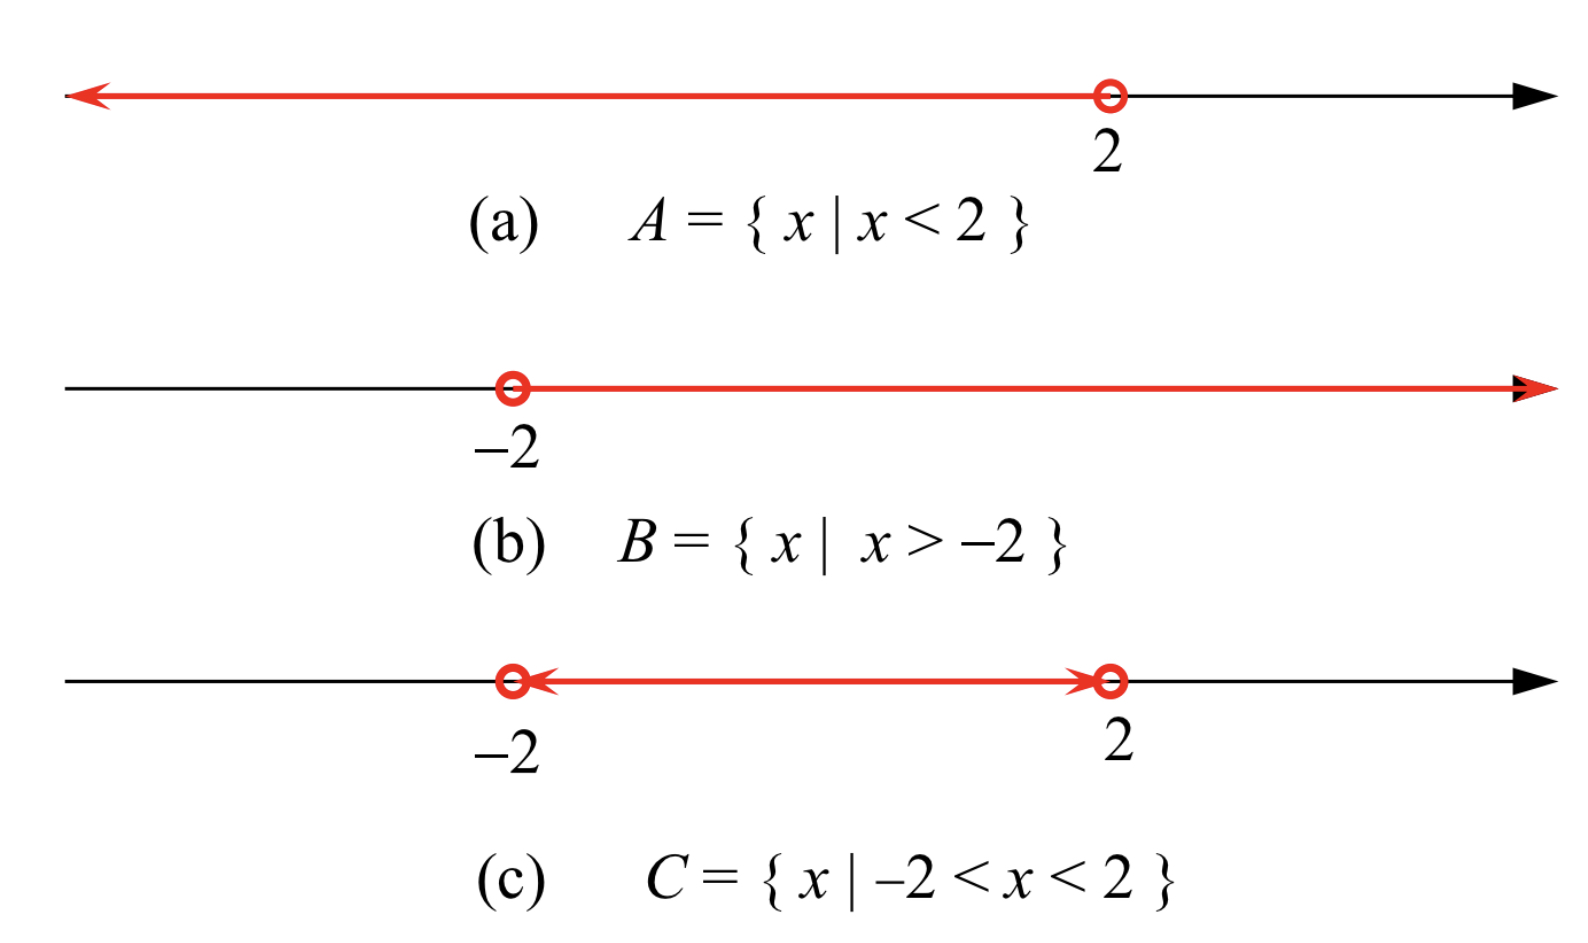
\includegraphics[scale=0.2]{Picture5.png}

\caption{  The sets $A$, $B$, $C$ in Example \ref{23020705}.}\label{figure5}
\end{figure}

If $S$ is a set of real numbers, the {\bf negative} of $S$, denoted by $-S$, is the set
\[-S=\left\{-x\,|\,x\in S\right\}.\]
For example, the set $B=\left\{x\,|\, x>-2\right\}$ is the negative of the set $\di A=\left\{x\,|\, x<2\right\}$, the set $\di C=\left\{x\,|\, -2<x<2\right\}$ is the negative of itself (see Figure \ref{figure5}). It is obvious that $S$ is bounded above if and only if $-S$ is bounded below.


Next, we recall the definition of maximum and minimum of a set.
\begin{definition}{Maximum and Minimum} Let $S$ be a nonempty subset of real numbers. 
\begin{enumerate}[1.]
\item  A number $c$ is called the {\bf largest element} or {\bf maximum} of $S$ if $c$ is an element of $S$ and
\[x\leq c\hspace{1cm}\text{for all}\;x\in S.\]
If the maximum of the set $S$ exists, we denote is by $\max S$.
\item A number $b$ is called the {\bf smallest element} or  {\bf minimum} of $S$ if $b$ is an element of $S$ and
\[x\geq b\hspace{1cm}\text{for all}\;x\in S.\]
If the minimum of the set $S$ exists, we denote it by $ \min S$.
\end{enumerate}
\end{definition}

Obviously, $b$ is the maximum of a set $S$ if and only if $-b$ is the minimum of the set $-S$.

\begin{example}{}
For the set $S_1=[-2,2]$, $-2$ is the minimum, and $2$ is the maximum.
\\
For the set $S_2=[-2, 2)$, $-2$ is the minimum, and there is no maximum.
\end{example}

This example shows that a bounded set does not necessarily have maximum or minimum.
However, a finite set always have a maximum and a minimum.

\begin{proposition}{}

If $S$ is a finite set, then $S$ has a maximum and a minimum.
\end{proposition}

 
Next, we introduce the concept of least upper bound.
\begin{definition}{Least Upper Bound}
Let $S$ be a nonempty subset of real numbers
 that is bounded above, and let $U_S$ be the set of upper bounds of $S$. Then $U_S$ is a nonempty set that is bounded below. If $U_S$ has a smallest element $u$, we say that $u$ is the {\bf least upper bound} or {\bf supremum} of $S$, and denote it by
\[u=\sup S.\]
 

\end{definition}
\begin{example}{}
For the sets $S_1=[-2,2]$ and  $S_2=[-2, 2)$, \[\sup S_1=\sup S_2=2.\]
\end{example}

Notice that $\sup S$, if exists, is not necessary an element of $S$.  The following proposition depicts the relation between the maximum of a set (if exists) and its least upper bound.
\begin{proposition}[label=23020606]{Supremum and Maximum}
Let $S$ be a nonempty subset of real numbers. Then $S$ has a maximum if and only if $S$ is bounded above and $\sup S$ is in $S$.
\end{proposition}

One natural question to ask is, if $S$ is a nonempty subset of real numbers that is bounded above, does $S$ necessarily have a least upper bound. The completeness axiom   asserts that this is true.
\begin{highlight}{Completeness Axiom}
If $S$  is a nonempty subset of real numbers that is bounded above, then $S$ has a least upper bound.
\end{highlight}

The reason this is formulated as an axiom is we cannot prove this   from our intuitive definition of real numbers. Therefore, we will assume this as a fact for the set of real numbers. A lots of theorems that we  are going to derive later is a consequence of this axiom. 

Actually, the set of real numbers can be constructed axiomatically, taken it to be a set that contains the set of rational numbers, satisfying all properties of addition and multiplication operations, as well as   the completeness axiom. However, this is a tedious construction and will drift us too far. 

 To show that the completeness axiom is not completely trivial, we  show in Example \ref{ex23020101} that if we only consider the set of rational numbers, we can find a subset of rational numbers $A$ that is bounded above but does not   have a least upper bound in the set of rational numbers. We look at the following example first.


\begin{example}[label=23020701]{}
Define the set of real numbers $S$ by
\[S=\left\{x\in \mathbb{R}\,|\, x^2<2\right\}.\]
Show that $S$ is nonempty and is bounded above. Conclude that the set 
\[A=\left\{x\in \mathbb{Q}\,|\, x^2<2\right\}\] is also nonempty and is bounded above by a rational number.
\end{example}

\begin{solution}{Solution}
 The number 1 is  in $S$, and so $S$ is nonempty.
For any $x\in S$, 
$x^2<2<4$, and hence
$x<2$.
This shows that $S$ is bounded above by 2.  
Since 1 and 2 are rational numbers, the same reasoning shows that the set $A$ is nonempty and is bounded above by a rational number.
\end{solution}
 
\begin{example}[label=ex23020101]{}
Consider the set 
\[A=\left\{x\in\mathbb{Q}\,|\, x^2<2\right\}.\]
By Example \ref{23020701},  $A$ is a nonempty subset of rational numbers that is bounded above by 2.
Let $U_A$ be the set of upper bounds of $A$ in $\mathbb{Q}$. Namely,
\[U_A=\left\{c\in\mathbb{Q}\,|\, x\leq c\;\text{for all}\;x\in A\right\}.\]
Show that $U_A$ does not have a smallest element.
\end{example}
\begin{solution}{Solution}
We use proof by contradiction. Assume that $U_A$ has a smallest element $c_1$, which is an upper bound of $A$ that is smaller than or equal to any upper bound of $A$. Then for any $x\in A$, 
\[x^2\leq c_1.\] 
 Since $1$ is in $A$,  $c_1$ is a positive rational number. Hence, there are poitive integers $p$ and $q$ such that
\[c_1=\frac{p}{q}.\]

Since there are no rational numbers whose square is 2, we must have either $c_1^2<2$ or $c_1^2>2$.  
 
Define the positive rational  number $c_2$ by
\[c_2=\frac{2p+2q}{p+2q}.\]


Notice that
\[c_1-c_2=\frac{p(p+2q)-q(2p+2q)}{q(p+2q)}=\frac{p^2-2q^2}{q(p+2q)},\]

\[c_1^2-2=\frac{p^2-2q^2}{q^2},\]
and 
\[c_2^2-2=\frac{4p^2+8pq+4q^2-2(p^2+4pq+4q^2)}{(p+2q)^2}=\frac{2(p^2-2q^2)}{(p+2q)^2}.\]


\textbf{Case 1: } $c_1^2<2$.\\
In this case, $p^2<2q^2$. It follows that $c_1<c_2$ and $c_2^2<2$. But then $c_1$ and $c_2$ are both in $A$, and $c_2$ is an element in $A$ that is larger than $c_1$, which contradicts to $c_1$ is an upper bound of $A$. Hence, we cannot have $c_1^2<2$.
\bs

\textbf{Case 2: } $c_1^2>2$.\\
In this case, $p^2>2q^2$. It follows that $c_1>c_2$ and $c_2^2>2$. 
Since $c_2^2>2$, we find that for any $x\in A$, \[x^2<2<c_2^2.\]Thus, 
\[-c_2<x<c_2.\] In particular, $c_2$ is also an upper bound of $A$. Namely, $c_2$ is in $U_A$.
But then $c_1$ and $c_2$ are both in $U_A$ and $c_1>c_2$. This contradicts to $c_1$ is the smallest element in $U_A$. Hence, we cannot have $c_1^2>2$.


Since both Case 1 and Case 2 lead to contradictions, we conclude that $U_A$ does not have a smallest element.
\end{solution}

In the solution above, the construction of the positive rational number $c_2$ seems a bit adhoc. In fact, we can define $c_2$ by
\[c_2=\frac{m p+2n q}{n p+m q}\]for any positive integers $m$ and $n$ with $m^2>2n^2$. Then the proof still works.

Now let us see how completeness axiom is used to guarantee that there is a real number whose square is 2. 

\begin{example}[label=23021011]{}
Use completeness axiom to show that there is a positive real number $c$ such that 
\[c^2=2.\]
\end{example}

\begin{solution}{Solution}
Define the set of real numbers $S$ by
\[S=\left\{x\in \mathbb{R}\,|\, x^2<2\right\}.\] Example \ref{23020701} asserts that $S$ is a nonempty subset of real numbers that is bounded above.
Completeness axiom  asserts that $S$ has a least upper bound $c$.\bs
Since $1$ is in $S$, $c\geq 1$.
We are going to prove that $c^2=2$   using proof by contradiction. If $c^2\neq 2$, then $c^2<2$ or $c^2>2$.


\textbf{Case 1:} $c^2<2$. \\
Let $d=2-c^2$. Then $0<d\leq 1$. Define the number $c_1$ by
\[c_1= c+\frac{d}{4c}.\]
Then $c_1>c$, and
\[c_1^2=c^2+\frac{d}{2}+\frac{d^2}{16c^2}\leq c^2+\frac{d}{2}+\frac{d}{16}<c^2+d=2.\]
This implies that $c_1$ is an element of $S$ that is larger than $c$, which contradicts to $c$  is an upper bound of $S$.

\textbf{Case 2:} $c^2>2$. \\
Let $d=c^2-2$. Then $d>0$. Define the number $c_1$ by
\[c_1= c-\frac{d}{2c}.\]
Then $c_1<c$, and
\[c_1^2=c^2-d+\frac{d^2}{4c^2}>c^2-d=2.\]
This implies that $c_1$ is an upper bound of $S$ that is smaller than $c$, which contradicts to $c$ is the least upper bound of $S$.

Since we obtain a contradiction if $c^2\neq 2$, we must have $c^2=2$.
\end{solution}
In fact, the completeness axiom can be used to show that for any positive real number $a$, there is a positive  real number $c$ such that 
\[c^2=a.\] We denote this number $c$ as $\sqrt{a}$, called the positive square root of $a$. The number $b=-\sqrt{a}$ is another real number such that $b^2=a$.

More generally, if $n$ is a positive integer, $a$ is a positive real number, then there is a positive real number $c$ such that $c^n=a$. We denote this number $c$ by
\[c=\sqrt[n]{a},\]called the positive $n^{\text{th}}$-root of $a$.

Using the interplay between a set and its negative, we can define the greatest lower bound of a set that is bounded below. 
 
\begin{definition}{Greatest Lower Bound}
Let $S$ be a nonempty subset of real numbers
 that is bounded below, and let $L_S$ be the set of lower bounds of $S$. Then $L_S$ is a nonempty set that is bounded above. If $L_S$ has a largest element $\ell$, we say that $\ell$ is the {\bf greatest lower bound} or {\bf infimum} of $S$, and denote it by
\[\ell=\inf S.\]
 

\end{definition}

From the completeness axiom, we have the following.
\begin{theorem}{}
If $S$ is a nonempty subset of real numbers
 that is bounded below, then $S$ has a greatest lower bound.
\end{theorem}

For a nonempty set $S$ that is bounded, it has a least upper bound $\sup S$ and a greatest lower bound $\inf S$. The following is quite obvious.

\begin{proposition}{}
If $S$ is a bounded nonempty subset of real numbers, it has a least upper bound $\sup S$ and a greatest lower bound $\inf S$. Moreover,
\[\inf S\leq \sup S,\]
and $\inf S=\sup S$ if and only if $S$ contains exactly one element.
\end{proposition}


Let us emphasize again the characterization of the least upper bound and greatest lower bound of a set.
\begin{highlight}{Characterization of Supremum and Infimum}
Let $S$ be a nonempty subset of real numbers, and let $a$ be a real number.
\begin{enumerate}[1.]
\item$a=\sup S$ if and only if the following two conditions are satisfied.
\begin{enumerate}[(i)]
\item For all $x\in S$, $x\leq a$.
\item If $b$ is a real number such that $x\leq b$ for all $x\in S$, then $a\leq b$.

\end{enumerate}
\item $a=\inf S$ if and only if the following two conditions are satisfied.
\begin{enumerate}[(i)]
\item For all $x\in S$, $x\geq a$.
\item If $b$ is a real number such that $x\geq b$ for all $x\in S$, then $a\geq b$.

\end{enumerate}
\end{enumerate}
\end{highlight}





\begin{example}{}
For each of the following set of real numbers, determine whether it has a least upper bound, and whether it has a greatest lower bound.  
\begin{enumerate}[(a)]
\item $A=\left\{x\in\mathbb{R}\,|\, x^3<2\right\}$
\item $B=\left\{x\in\mathbb{R}\,|\, x^2<10\right\}$.
\end{enumerate}
\end{example}
\begin{solution}{Solution}
\begin{enumerate}[(a)]
\item The set $A$ is bounded above, since if $x\in A$, then $x^3<2<2^3$, and so $x<2$. The set $A$ is not bounded below since it contains all negative numbers. Hence, $A$ has a least upper bound, but it does not have a greatest lower bound.
\item If $x^2<10$, then $x^2<16$, and so $-4<x<4$. This shows that $B$ is bounded. Hence, $B$ has a least upper bound, and a greatest lower bound.
\end{enumerate}
\end{solution}

Finally, we want to highlight again Proposition \ref{23020606} together with its lower bound versus infimum counterpart.
\begin{highlight}{Existence of Maximum and Minimum}
Let $S$ be a nonempty subset of real numbers. 
\begin{enumerate}[1.]
\item $S$ has a maximum if and only if $S$ is bounded above and $\sup S$ is in $S$.
\item $S$ has a minimum if and only if $S$ is bounded below and $\inf S$ is in $S$.
\end{enumerate}
\end{highlight}
\vp
 
\noindent
{\bf \large Exercises  \thesection}
\setcounter{myquestion}{1}

 \begin{question}{\themyquestion}
For each of the following sets of real numbers, find its least upper bound,   greatest lower bound,  maximum, and minimum if any of these  exists. If any of these does not exist, explain why.
\begin{enumerate}[(a)]
\item
$A=(-\infty, 20)$
\item $B=[-3, \infty)$
\item $C=[-10, -2)\cup (1, 12]$
\item $D=[-2, 5]\cap (-1, 7]$
\end{enumerate}
\end{question}

\atc
 \begin{question}{\themyquestion}
 Use completeness axiom to show that there is a positive real number $c$ such that 
\[c^2=5.\]
\end{question}
\atc
 \begin{question}{\themyquestion}
For each of the following set of real numbers, determine whether it has a least upper bound, and whether it has a greatest lower bound.  
\begin{enumerate}[(a)]
\item $A=\left\{x\in\mathbb{R}\,|\, x^3>10\right\}$
\item $B=\left\{x\in\mathbb{R}\,|\, x^2<2020\right\}$.
\end{enumerate}
\end{question}

\vp
\section{Distributions of Numbers }\label{sec1.4}
In this section, we consider additional properties of the set of integers, rational numbers and real numbers.

We start by a proposition about distribution of integers.
\begin{proposition}
{}
\begin{enumerate}[1.]
\item If $n$ is an integer, there is no integer in the interval $(n, n+1)$.
\item For any real number $c$, there is exactly one integer in the interval $[c, c+1)$, and there is exactly one integer in the interval $(c, c+1]$.

\end{enumerate}
\end{proposition}
These statements are quite obvious. For any real number $c$, the integer in the interval $[c, c+1)$ is  $\lceil c\rceil$, called the {\bf ceiling} of $c$. It is the smallest integer larger than or equal to $c$. For example $\lceil -2.5\rceil=-2$, $\lceil -3\rceil =-3$. The integer in the interval $(c, c+1]$ is $\lfloor c\rfloor+1$, where $\lfloor c\rfloor$ is the {\bf floor} of $c$.  It is the largest integer that is less than or equal to $c$. For example, $\lfloor -2.5\rfloor =-3$, $\lfloor -3\rfloor =-3$.

In Section \ref{sec1.3}, we have seen that a nonempty subset of real numbers that is bounded above does not necessary have a maximum. Example \ref{ex23020101} shows that a nonempty  subset of rational numbers that is bounded above also does not necessary have a maximum. However, for nonempty  subsets of integers, the same is not true.

\begin{proposition}{}
Let $S$ be a nonempty subset of integers.
\begin{enumerate}[1.]
\item If $S$ is bounded above, it has a maximum.
\item If $S$ is bounded below, it has a minimum.
\end{enumerate}
\end{proposition}

The two statements are equivalent, and the second statement is a generalization of the well-ordered principle for the set of positive integers. It can be proved using mathematical induction.


Next we discuss another important property called the Archimedean property. First let us show that the set of positive integers $\mathbb{Z}^+$ is not bounded above. 

\begin{theorem}
[label=thm23020202]{}The set of positive integers $\mathbb{Z}^+$ is not bounded above. 
\end{theorem}
\begin{myproof}{Proof}
Assume to the contrary that the set of positive integers $\mathbb{Z}^+$ is bounded above. By completeness axiom, it has a least upper bound $u$. 
Since $u-1<u$, $u-1$ is not an upper bound of $\mathbb{Z}^+$. Hence, there is a positive integer $n$ such that
\[n>u-1.\]
It follows that
\[n+1>u.\]
 Since $n+1$ is also a positive integer, this says that there is an element of $\mathbb{Z}^+$ that is larger than the least upper bound of $\mathbb{Z}^+$. This contradicts to the definition of least upper bound. Hence, $\mathbb{Z}^+$ cannot be bounded above.
\end{myproof}
The proof uses the key fact  that any number that is smaller than the least upper bound of a set is not an upper bound of the set. This is a standard technique in proofs.

\begin{theorem}{The Archimedean Property}
\begin{enumerate}[1.]
\item
For any positive number $M$, there is a positive integer $n$ such that $n> M$.
\item For any positive number $\varepsilon$, there is a positive integer $n$ such that $1/n<\varepsilon$.
\end{enumerate}
\end{theorem}
These two statements are equivalent, and the first statement is equivalent to the fact that the set of positive integers is not bounded above.
 
 In the following, we consider another property called denseness.
\begin{definition}{Denseness}
Let $S$ be a subset of real numbers. We say that $S$ is {\bf dense} in $\mathbb{R}$ if every open interval $(a, b)$ contains an element of $S$.
\end{definition}

A key fact we want to prove is that the set of rational numbers $\mathbb{Q}$ is dense in the set of real numbers. 

\begin{theorem}{Denseness of the Set of Rational Numbers}
The set of rational numbers $\mathbb{Q}$ is dense in the set of real numbers $\mathbb{R}$.

\end{theorem}
\begin{myproof}{Proof}
Let $(a, b)$ be an open interval. Then $\varepsilon=b-a>0$. By the Archimedean property, there is a positive integer $n$ such that
 $1/n <\varepsilon$.  Hence, \[nb-na=n\varepsilon>1,\]and so
\[ na+1<nb.\]
Consider the interval $(na, na+1]$. There is an integer $m$ that lies in this interval. In other words,
\[na<m\leq na+1<nb.\]
Dividing by $n$, we have
\[a<\frac{m}{n}<b.\]
This proves that the open interval $(a,b)$ contains the rational number $m/n$, and thus completes the proof that the set of rational numbers is dense in the set of real numbers.
\end{myproof}

Recall that a set $A$ is said to be   {\bf countably infinite} if there is a bijection $f:  \mathbb{Z}^+\to A$. A set that is either finite or countably infinite is said to be {\bf countable}.  We assume that students have seen the proofs of the following.


\begin{proposition}{}
The set of integers $\mathbb{Z}$ and the set of rational numbers $\mathbb{Q}$ are countable, while the set of real numbers $\mathbb{R}$ is not countable.
\end{proposition}

Since the union of countable sets is  countable, this proposition implies that the set of irrational numbers is uncountable. Therefore, there are far more irrational numbers than rational numbers. Hence, it should not be surprising that the set of irrational numbers is also dense in the set of real numbers. To prove this, 
let us recall the following facts.
\begin{highlight}{Rational Numbers and Irrational Numbers}
\begin{enumerate}[1.]
\item
If $a$ and $b$ are rational numbers, then $a+b$ and $ab$ are rational numbers.
\item If $a$ is a nonzero rational number, $b$ is an irrational number, then $ab$ is an irrational number.
\end{enumerate}
\end{highlight}

\begin{theorem}{Denseness of the Set of Irrational Numbers}
The set of irrational numbers $\mathbb{R}\setminus\mathbb{Q}$ is dense in the set of real numbers $\mathbb{R}$.

\end{theorem}
\begin{myproof}{Proof}
Let $(a, b)$ be an open interval.  Define
\[c=\frac{a}{\sqrt{2}}, \hspace{1cm}d=\frac{b}{\sqrt{2}}.\]
Then $c<d$. By the denseness of rational numbers, there is a rational number $u$ that lies in the interval $(c,d)$. Hence, 
\[\frac{a}{\sqrt{2}}=c<u<d=\frac{b}{\sqrt{2}}.\]
Let $v=\sqrt{2}u$. Then $v$ is an irrational number satisfying
\[a<v<b.\]
This proves that the open interval $(a, b)$ contains the irrational number $v$, and thus completes the proof that the set of irrational numbers is dense in the set of real numbers.
\end{myproof}

 
\begin{example}{}
Is the set of integers $\mathbb{Z}$ dense in $\mathbb{R}$? Justify your answer.
\end{example}
\begin{solution}{Solution}
$(0,1)$ is an open interval that does not contain any integers. Hence, the set of integers is not dense in $\mathbb{R}$.
\end{solution}
\vspace{0.8cm}
\hrule
\vspace{0.8cm}
\noindent
{\bf \large Exercises  \thesection}
\setcounter{myquestion}{1}


 \begin{question}{\themyquestion}
Let  $S=\mathbb{Q}\setminus\mathbb{Z}$. Is the set $S$ dense in $\mathbb{R}$? Justify your answer.
\end{question}

\vp
\section{The Convergence of Sequences}\label{sec1.5}

{\bf Infinite sequences} play important roles in analysis. We will consider infinite sequences that are indexed by the set of positive integers
\[a_1, a_2, \ldots, a_n, \ldots\]
This can be considered as a function $f:\mathbb{Z}^+\rightarrow\mathbb{R}$, where $a_n=f(n)$.  The general term in the sequence is denoted by $a_n$.  In some occasions, we may also want to consider sequences that start with $a_0$.

In the sequel, when we say a sequence, we always mean an infinite sequence that is indexed by the set of positive integers, unless otherwise specified.
A sequence can be denoted by $\{a_n\}$ or $\{a_n\}_{n=1}^{\infty}$. This should not be confused with the set $\{a_n\,|\, n\in\mathbb{Z}^+\}$ that contains all terms in the sequence. 

There are various ways to specify a sequence. One of the ways is to give an explicit formula for the general term $a_n$. For example $\{1/n\}$ is the sequence with $a_n=1/n$. More precisely, it is the sequence with first five terms given by
\[1, \frac{1}{2}, \frac{1}{3}, \frac{1}{4}, \frac{1}{5}, \ldots.\]
A sequence can also be defined recursively, such as the following example. 

\begin{example}[label=ex23020301]{}
Let $\{a_n\}$ be the sequence defined by $a_1=2$, and for $n\geq 2$,
\[a_n=a_{n-1}+3.\]
  Find the first 5 terms of the sequence.
\end{example}
\begin{solution}{Solution}We compute recursively.\\
$
a_1 =2 $\\
$a_2= a_1+3=5 $\\
$a_3 =a_2+3=8$\\
$a_4 =a_3+3=11$\\
$a_5 =a_4+3=14$
 
\end{solution}
The sequence $\{a_n\}$ in Example \ref{ex23020301} is  an example of an arithmetic sequence. One can prove by induction that
\[a_n=3n-1.\]

\begin{example}[label=ex23020302]{}
Let $\{s_n\}$ be the sequence defined by $s_1=\frac{1}{2}$, and for $n\geq 2$,
\[s_n=s_{n-1}+\frac{1}{2^n}.\]
  Find the first 5 terms of the sequence.
\end{example}
\begin{solution}{Solution}We compute recursively.
\begin{align*}
s_1&=\frac{1}{2} \\
s_2&=s_1+\frac{1}{2^2} =\frac{3}{4}  \hspace{8cm}\\
s_3&=s_2+\frac{1}{2^3} =\frac{7}{8}\\
s_4&=s_3+\frac{1}{2^4} =\frac{15}{16} \\
s_5&=s_4+\frac{1}{2^5} =\frac{31}{32} \hspace{8cm}
\end{align*}
\end{solution}
The sequence $\{s_n\}$ in Example \ref{ex23020302} is the partial sum of the geometric sequence $\di\left\{\frac{1}{2^n}\right\}$. One can prove by induction that
\[s_n=1-\frac{1}{2^n}.\]
\begin{example}[label=ex23020303]{}
Let $\{s_n\}$ be the sequence defined by 
\[s_n=1+\frac{1}{2}+\cdots+\frac{1}{n}.\]
  This sequence can also be defined recursively by $s_1=1$, and for $n\geq 2$,
\[s_n=s_{n-1}+\frac{1}{n}.\]
\end{example}For the sequence $\{s_n\}$ defined in Example \ref{ex23020303}, the general term $s_n$ cannot be expressed as an explicit elementary function of $n$.

\begin{example}[label=ex23020304]{}
Let $\{a_n\}$ be the sequence defined by $a_1=2$, and for $n\geq 1$,
\[a_{n+1}=\begin{cases} a_n+\frac{1}{n}\quad &\text{if}\;a_n<3,\\a_n-\frac{1}{n}\quad &\text{if}\;a_n\geq 3.\end{cases}\]
Find the first six terms of the sequence.
\end{example}
\begin{solution}{Solution}We compute recursively.
\begin{align*}
a_1&=2<3\\
a_2&= a_1+1=3\geq 3 \\
a_3&=a_2-\frac{1}{2}=\frac{5}{2}<3\\
a_4&=a_3+\frac{1}{3}=\frac{17}{6}<3\\
a_5&=a_4+\frac{1}{4}=\frac{37}{12}\geq 3\hspace{8cm}
\\
a_6&=a_5-\frac{1}{5}=\frac{173}{60}
\end{align*}
\end{solution}


From the examples above, we observe that some sequences are monotone. 

\begin{definition}{Increasing and Decreasing Sequences}
\begin{enumerate}[1.]
\item
We say that a sequence $\{a_n\}$ is {\bf increasing} if
\[a_n\leq a_{n+1}\hspace{1cm}\text{for all}\;n\in\mathbb{Z}^+.\]
\item We say that a sequence is {\bf decreasing} if 
\[a_n\geq a_{n+1}\hspace{1cm}\text{for all}\;n\in\mathbb{Z}^+.\]
\item We say that a sequence $\{a_n\}$ is {\bf monotone} if it is an increasing sequence or it is a decreasing sequence.
\end{enumerate}
\end{definition}

\begin{example}{}
\begin{enumerate}[1.]
\item The sequence  $\{a_n\}$ defined in Example \ref{ex23020301} is increasing.
\item The sequence $\di\left\{\frac{1}{n}\right\}$ is decreasing.
\item The sequence  $\{a_n\}$ defined in Example \ref{ex23020304} is neither increasing nor decreasing.

\end{enumerate}
\end{example}

 

In analysis, we are often led to consider the behavior of a sequence $\{a_n\}$ when $n$ gets larger than larger. We are interested to know whether the sequence would approach a fixed value. This leads to the idea of convergence.

\begin{definition}{Convergence of   Sequences}
A sequence $\{a_n\}$ is said to {\bf converge} to the number $a$ if for every positive number $\varepsilon$, there is a positive integer $N$ such that for all $n\geq N$, 
\[|a_n-a|<\varepsilon.\] 
\end{definition}
Here the positive number $\varepsilon$ is used to measure the distance from the term $a_n$ to the number $a$. Since $\varepsilon$ can be any positive number, the distance can get as small as possible. 

 \begin{figure}[ht]
\centering
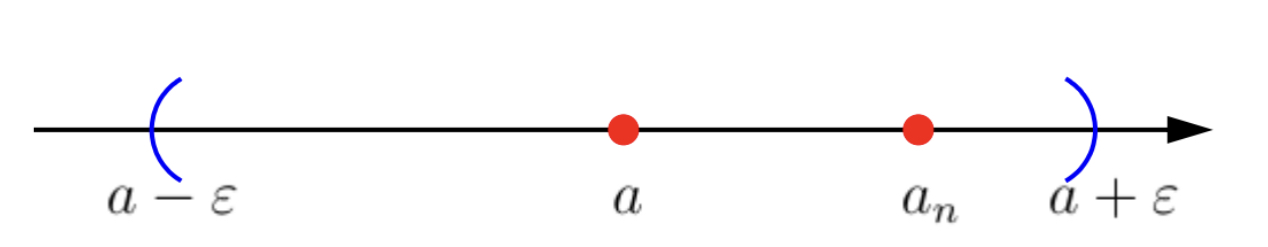
\includegraphics[scale=0.2]{Picture2.png}

\caption{  $|a_n-a|<\varepsilon$.}\label{figure2}
\end{figure}

One question that is natural to ask is whether a sequence $\{a_n\}$ can converge to two different numbers. This is   impossible.
\begin{theorem}[label=thm23020301]{}
A sequence cannot converge to two different numbers.
\end{theorem}
\begin{myproof}{Proof}
This is proved by contradiction. Assume that there is a sequence $\{a_n\}$ which converges to two different numbers $b$ and $c$.  Let
\[\varepsilon=\frac{|b-c|}{2}.\]
Since $b$ and $c$ are distinct, $|b-c|>0$ and so $\varepsilon>0$. By definition of convergence, there is a positive integer $N_1$ such that for all $n\geq N_1$,
\[|a_n-b|<\varepsilon.\]
Similarly, there is a positive integer $N_2$ such that for all $n\geq N_2$, 
\[|a_n-c|<\varepsilon.\]
If $N=\max\{N_1, N_2\}$, then $N\geq N_1$ and $N\geq N_2$. It follows that
\[|b-c|=|(a_N-c)-(a_N-b)|\leq |a_N-c|+|a_N-b|<\varepsilon+\varepsilon=|b-c|.\]
This gives $|b-c|<|b-c|$, which is a contradiction. Hence, we conclude that a sequence cannot converge to two different numbers.
\end{myproof}
\begin{figure}[ht]
\centering
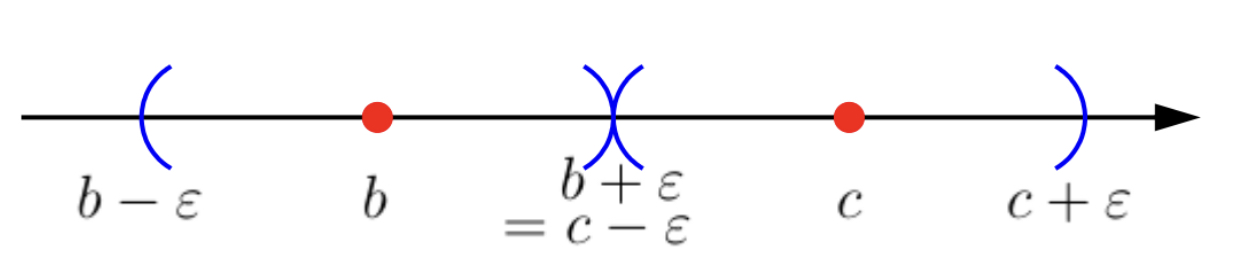
\includegraphics[scale=0.2]{Picture3.png}

\caption{ A sequence $\{a_n\}$ cannot converge to two different numbers $b$ and $c$.}\label{figure3}
\end{figure}

\begin{highlight}{Limit of a Sequence}
If a sequence $\{a_n\}$ converges to a number $a$, we say that the sequence is \textbf{convergent}. Otherwise, we say that it is \textbf{divergent}. Theorem \ref{thm23020301} says that for a convergent sequence $\{a_n\}$, the number $a$ that it converges to is unique. We call this unique number $a$ the \textbf{limit} of the convergent sequence $\{a_n\}$, and express the convergence of $\{a_n\}$ to $a$ as
\[\lim_{n\rightarrow\infty}a_n=a.\]

\end{highlight}


Using logical expression,     
\begin{highlight}{}
\[\lim_{n\rightarrow\infty}a_n=a\;\iff\; \forall \varepsilon>0, \;\exists N\in \mathbb{Z}^+, \;\forall n\geq N,\; |a_n-a|<\varepsilon.\]
 \end{highlight}
Let us look at a simple example of a constant sequence.

\begin{example}{}
Let $c$ be a real number and let $\{a_n\}$ be the sequence with $a_n=c$ for all $n\in\mathbb{Z}^+$. Then for any $\varepsilon>0$, we take $N=1$. For all $n\geq N=1$, we have
\[|a_n-c|=|c-c|=0<\varepsilon,\] which shows that
the limit of the constant sequence $\{a_n\}$   is $c$. Namely,
\[\lim_{n\rightarrow\infty}c=c.\]

\end{example}
Another simple example is the sequence $\{a_n\}$ with $\di a_n=\frac{1}{n}$.
\begin{example}[label=ex23020305]{}
Use the definition of convergence to show that 
\[\lim_{n\rightarrow\infty}\frac{1}{n}=0.\]
\end{example}
\begin{solution}{Solution}
Given $\varepsilon>0$, the Archimedean property asserts that there is a positive integer $N$ such that $1/N<\varepsilon$. If $n\geq N$, we have   
\[0<\frac{1}{n}\leq\frac{1}{N}<\varepsilon.\] 
This gives
\[\left|\frac{1}{n}-0\right|<\varepsilon\hspace{1cm}\text{for all}\;n\geq N.\]
By definition, we conclude that
\[\lim_{n\rightarrow\infty}\frac{1}{n}=0.\]
\end{solution}



Let $f:\mathbb{Z}^+\rightarrow\mathbb{Z}^+$ be a function satisfying
\[f(k)<f(k+1)\hspace{1cm}\text{for all}\;k\in \mathbb{Z}^+.\]
Then $f(\mathbb{Z}^+)$ is an infinite set of positive integers.   If we let
$n_k=f(k)$, then
\[n_1<n_2<n_3<\cdots.\]Namely, $n_1, n_2, n_3, \ldots$ is a strictly increasing sequence of positive integers. 
\begin{definition}{Subsequence}
Let $\{a_n\}$ be a sequence. A subsequence of $\{a_n\}$ is a sequence $\{a_{n_k}\}$ indexed by $k\in\mathbb{Z}^+$, where $n_k=f(k)$ is defined by a function $f:\mathbb{Z}^+\rightarrow\mathbb{Z}^+$  satisfying
\[f(k)<f(k+1)\hspace{1cm}\text{for all}\;k\in \mathbb{Z}^+.\]
\end{definition}

\begin{example}{}
The sequence $\{1/(2n-1)\}$ with first three terms given by 
\[1, \frac{1}{3}, \frac{1}{5},\]
is a subsequence of the sequence $\{1/n\}$ whose first five terms are
\[1, \frac{1}{2}, \frac{1}{3}, \frac{1}{4}, \frac{1}{5}.\]
\end{example}

If a sequence $\{a_n\}$ converges to $a$, what can we say about its subsequence? It is natural to expect any subsequence of $\{a_n\}$ also converges to $a$.

\begin{theorem}[label=thm23020305]{Subsequence of a Convergent Sequence}
If the sequence $\{a_n\}$ converges to $a$, then any of its subsequence also converges to $a$.
\end{theorem}
\begin{myproof}{Proof}
Let $\{a_{n_k}\}$ be a subsequence of $\{a_n\}$. Notice that for all $k\in\mathbb{Z}^+$, 
\[n_k\geq k.\]
Given $\varepsilon>0$, there is a positive integer $N$ such that for all $n\geq N$,
\[|a_n-a|<\varepsilon.\]
Take $K=N$. Then for all $k\geq K$, $n_k\geq n_K=n_N\geq  N$, and thus,
\[|a_{n_k}-a|<\varepsilon.\] This proves that $\{a_{n_k}\}$ indeed converges to $a$.
\end{myproof}

\begin{example}
{}
Find the limit 
\[\lim_{n\rightarrow\infty}\frac{1}{2^n}\] if it exists.
\end{example}
\begin{solution}{Solution}
Notice that $\di\left\{\frac{1}{2^n}\right\}$ is a subsequence of $\di\left\{\frac{1}{n}\right\}$ with $n_k=2^k$. By Example \ref{ex23020305}, 
\[\lim_{n\rightarrow\infty}\frac{1}{n}=0.\] We conclude from Theorem \ref{thm23020305} that \[\lim_{n\rightarrow\infty}\frac{1}{2^n}=0.\]
\end{solution}

\begin{example}{}
Show that the sequence $\{(-1)^n\}$ is divergent.
\end{example}
\begin{solution}{Solution}
Let $a_n=(-1)^n$. Then  for any positive integer $n$, $a_{2n-1}=-1$, and $a_{2n}=1$. The subsequence $\{a_{2n-1}\}$ of $\{a_n\}$ converges to $-1$, while the subsequence  $\{a_{2n}\}$ of $\{a_n\}$ converges to 1. Since there are two subsequences of $\{a_n\}$ that converge to two different limits, by Theorem \ref{thm23020305}, the sequence $\{a_n\}$ is not convergent.
\end{solution}

For the sequence $\{a_n\}$ defined in Example \ref{ex23020301}, we can see that the set $\{a_n\,|\, n\in \mathbb{Z}^+\}$ is not bounded above. Therefore, we would expect that the sequence does not converge to any number.

For simplicity, we say that a sequence $\{a_n\}$ is bounded above/bounded below/ bounded if the set $\{a_n\,|\, n\in \mathbb{Z}^+\}$  is bounded above/bounded below/bounded . If  the sequence $\{a_n\}$ is bounded above, we denote the supremum of the set $\{a_n\,|\, n\in \mathbb{Z}^+\}$  as $\sup\{a_n\}$. If  the sequence $\{a_n\}$ is bounded below, we denote the infimum of the set $\{a_n\,|\, n\in \mathbb{Z}^+\}$  as $\inf\{a_n\}$. 

We have the following theorem which guarantees that a convergent sequence must be bounded.

\begin{theorem}[label=thm23020304]{Boundedness of Convergent Sequence}
If a sequence $\{a_n\}$ is convergent, then it is bounded. Equivalently, if a sequence $\{a_n\}$ is not bounded, then it is not convergent.
\end{theorem}
\begin{myproof}{Proof}
Let $\{a_n\}$ be a convergent sequence that converges to the limit $a$. By definition of convergence with $\varepsilon=1$, there is a positive integer $N$ such that for all $n\geq N$,
\[|a_n-a|<1.\]
This implies that
\[|a_n|\leq |a_n-a|+|a|<1+|a|\hspace{1cm}\text{for all}\;n\geq N.\]
Define
\[M=\max\left\{|a_1|, |a_2|, \ldots, |a_{N-1}|, |a|+1\right\}.\]Then 
\[|a_n|\leq M\hspace{1cm}\text{for all}\;n\in \mathbb{Z}^+.\]This shows that the sequence $\{a_n\}$ is bounded.
\end{myproof}

\begin{example}{}
By Theorem  \ref{thm23020304},  the sequence $\{a_n\}$ defined in Example \ref{ex23020301} is not convergent.\end{example}

If the sequence $\{a_n\}$ is convergent, and $c$ is a constant, it is natural to expect that the sequence $\{ca_n\}$ is also convergent.  

\begin{proposition}[label=p23020401]{}
If the sequence $\{a_n\}$ converges to $a$, then the sequence $\{ca_n\}$ converges to $ca$.
\end{proposition}
\begin{myproof}{Proof}
  Given $\varepsilon>0$, the number\[\varepsilon_1=\di\frac{\varepsilon}{|c|+1}\] is also positive. Since $\{a_n\}$ converges to $a$, there is a positive integer $N$ such that for all $n\geq N$,
\[|a_n-a|<\varepsilon_1=\frac{\varepsilon}{|c|+1}.\]
It follows that for all $n\geq N$,
\[|ca_n-ca|=|c||a_n-a|<\frac{|c|}{|c|+1}\varepsilon<\varepsilon.\]
This proves that $\{ca_n\}$ converges to $ca$.
\end{myproof}

\begin{example}{}
By Proposition \ref{p23020401}, we find that for any constant $c$,
\[\lim_{n\rightarrow\infty}\frac{c}{n}=0.\]
\end{example}
 


 In the following, we establish a comparison theorem for limits.
\begin{theorem}[label=squeeze]{Squeeze Theorem}
Let $\{a_n\}$, $\{b_n\}$ and $\{c_n\}$ be three sequences. Assume that there is a positive integer $N_0$ such that for all $n\geq N_0$,
\[b_n\leq a_n\leq c_n.\]
If both the sequences $\{b_n\}$ and $\{c_n\}$ converge to $\ell$, then the sequence $\{a_n\}$ also converges to $\ell$.
\end{theorem}

 

\begin{myproof}{ Proof }
 
For a positive number $\varepsilon$, since the sequence $\{b_n\}$ converges to $\ell$, there is a positive integer $N_1$ such that for all $n\geq N_1$, 
\[|b_n-\ell|<\varepsilon.\]
This implies that for all $n\geq   N_1$, 
\[  b_n-\ell>-\varepsilon.\]
Similarly, since the sequence $\{c_n\}$ converges to $\ell$, there is a positive integer $N_2$ such that for all $n\geq N_2$,
\[|c_n-\ell|<\varepsilon.\]
This implies that for all $n\geq N_2$, 
\[c_n-\ell<\varepsilon.\]
Let $N=\max\{N_0, N_1, N_2\}$. If $n\geq N$, $n\geq N_0$, $n\geq N_1$ and $n\geq N_2$. Therefore, if $n\geq N$,
\[a_n-\ell\geq b_n-\ell>-\varepsilon,\]and
\[a_n-\ell\leq c_n-\ell<\varepsilon.\]
This proves that for all $n\geq N$,
\[|a_n-\ell|<\varepsilon.\]Therefore, the sequence $\{a_n\}$ converges to $\ell$.
\end{myproof}


When applying the squeeze theorem, we are interested in the limit of the sequence $\{a_n\}$. It is not enough to find two seqeunces $\{b_n\}$ and $\{c_n\}$ satisfying
\[b_n\leq a_n\leq c_n\] for all $n$ greater than or equal to a fixed $N_0$. The two sequences $\{b_n\}$ and $\{c_n\}$ must have the same limit. 
\begin{example}{}
For the sequence $\{a_n\}$ with
\[a_n=\frac{(-1)^n}{n},\]
we have
\[-\frac{1}{n}\leq a_n\leq \frac{1}{n}.\]
Since
\[\lim_{n\rightarrow\infty}\frac{1}{n}=0,\]we have
\[\lim_{n\rightarrow\infty}-\frac{1}{n}=0.\]
By squeeze theorem, 
\[\lim_{n\rightarrow\infty}\frac{(-1)^n}{n}=0.\]
\end{example}

More generally, we have the following.
\begin{theorem}[label=thm23020307]{}
The sequence $\{a_n\}$ converges to 0 if and only if the sequence $\{|a_n|\}$ converges to 0.
\end{theorem}
 
A word of caution. If the sequence $\{|a_n|\}$ is convergent, the sequence $\{a_n\}$ is not necessarily convergent. An example is the sequence $\{a_n\}$ with $a_n=(-1)^n$. 
Theorem \ref{thm23020307} asserts that if $\{|a_n|\}$ converges to $0$, then $\{a_n\}$ is convergent, and it converges to 0.
Nevertheless, if the sequence $\{a_n\}$ is convergent, the sequence $\{|a_n|\}$ is necessarily convergent (see Question \ref{absolute}).
 
\begin{myproof}{\linkt Proof of Theorem \ref{thm23020307}\linko }
 
First assume that the sequence $\{a_n\}$ converges to 0. Given $\varepsilon>0$, there is a positive integer $N$ such that for all $n\geq N$,
\[|a_n-0|<\varepsilon.\]\bp
Notice that \[\bigl|\,|a_n|-0\,\bigr|=|a_n|=|\,a_n-0\,|.\]
  Hence, for all $n\geq N$,
\[\bigl|\,|a_n|-0\,\bigr|<\varepsilon.\]This proves that the sequence $\{|a_n|\}$ converges to 0.

Next, we assume that the sequence $\{|a_n|\}$ converges to 0. Then the sequence $\{-|a_n|\}$ also converges to 0. Since
\[-|a_n|\leq a_n\leq |a_n|,\]
 squeeze theorem implies that the sequence $\{a_n\}$ converges to 0.
\end{myproof}
 
In the following, we discuss two useful results that can be deduced from specific information about a convergent sequence. They will be useful in the proofs of other theorems that we are going to discuss.

\begin{lemma}[label=23020405]{Sequence with Positive Limit}
If $\{a_n\}$ is a sequence that converge to a positive number $a$, there is a positive integer $N$ such that $a_n>a/2>0$ for all $n\geq N$. 
\end{lemma}
One can easily formulate a counterpart of this lemma for a sequence with negative limit.
\begin{myproof}{Proof}
Take $\varepsilon=a/2$. Then $\varepsilon>0$. Hence, there is a positive integer $N$ so that for all $n\geq N$, 
\[|a_n-a|<\frac{a}{2}.\]
This implies that for all $n\geq N$,
\[a_n-a>-\frac{a}{2}.\]
Thus, for all $n\geq N$,
\[a_n>\frac{a}{2}>0.\]
\end{myproof}

\begin{lemma}[label=23020406]{}
\begin{enumerate}[1.]
\item
Given that $\{a_n\}$ is a sequence that is bounded above by $c$. If  $\{a_n\}$ converges to $a$, then $a\leq c$. 
\item 
Given that $\{a_n\}$ is a sequence that is bounded below by $b$. If  $\{a_n\}$ converges to $a$, then $a\geq b$. 
\item Given that $\{a_n\}$ is a sequence satifying
\[b\leq a_n\leq c\hspace{1cm}\text{for all}\; n\in\mathbb{Z}^+.\]If  $\{a_n\}$ converges to $a$, then $b\leq a\leq c$.
\end{enumerate}
\end{lemma}
It is suffices to prove the first statement. The second statement follows by considering the negative of the sequence. The third statement follows by combining the results of the first two statements.
\begin{myproof}{Proof}


Given that \[\di\lim_{n\rightarrow\infty}a_n=a\quad\text{and}\quad a_n\leq c \quad \text{for all}\;n\in\mathbb{Z}^+,\] we want to show that $a\leq c$. Assume to the contrary that $a>c$. Take $\varepsilon=a-c$. Then $\varepsilon>0$. By definition of convergence, there is a positive integer $N$ such that for all $n\geq N$,
\[|a_n-a|<\varepsilon.\]
This implies that
\[a_n-a>-\varepsilon=c-a\hspace{1cm}\text{when}\;n\geq N.\]
Hence,
\[a_n>c\hspace{1cm}\text{when}\;n\geq N.\]This contradicts to $a_n\leq c$ for all $n\in\mathbb{Z}^+$.
Therefore, we must have $a\leq c$.

\end{myproof}
 


In Proposition \ref{p23020401}, we have seen what happens when   a convergent sequence is multiplied by a constant. In the following, we   inspect the behaviour of limits with respect to sums, products and quotients.
We start by sums.
\begin{theorem}[label=23020402]{Sums of Convergent Sequences}
If the sequences $\{a_n\}$ and $\{b_n\}$ converge to $a$ and $b$ respectively, the sequence $\{a_n+b_n\}$ converges to $a+b$. 
\end{theorem}
\begin{highlight}{Linearity of Limits of Sequences}
 Combining Proposition \ref{p23020401} and Theorem \ref{23020402}, we obtain  the following. If
\[\lim_{n\rightarrow \infty}a_n=a,\hspace{1cm}\lim_{n\rightarrow\infty}b_n=b,\]then for any constants $\alpha$ and $\beta$,
\[\lim_{n\rightarrow\infty}\left(\alpha a_n+\beta b_n\right)=\alpha a+\beta b.\]  

 \end{highlight}
\begin{myproof}{\linkt Proof of Theorem \ref{23020402}\linko}
 
Given a positive number $\varepsilon$, the number $\varepsilon/2$ is also positive. Since the sequence $\{a_n\}$ converges to $a$, there is a positive integer $N_1$ such that for all $n\geq N_1$,
\[|a_n-a|<\frac{\varepsilon}{2}.\]
Similarly, 
 there is a positive integer $N_2$ such that for all $n\geq N_2$,
\[|b_n-b|<\frac{\varepsilon}{2}.\]
Take $N=\max\{N_1, N_2\}$. Then $N$ is a positive integer and $N\geq N_1$, $N\geq N_2$. If $n\geq N$, triangle inequality implies that
\begin{align*}
\left|(a_n+b_n)-(a+b)\right|&=|(a_n-a)+(b_n-b)|\\
&\leq |a_n-a|+|b_n-b|\\
&<\frac{\varepsilon}{2}+\frac{\varepsilon}{2}\\
&=\varepsilon.
\end{align*}This proves that the sequence $\{a_n+b_n\}$ converges to $a+b$.
\end{myproof}
 

Now we consider products.
\begin{theorem}[label=23020403]{Products of Convergent Sequences}
If the sequences $\{a_n\}$ and $\{b_n\}$ converge to $a$ and $b$ respectively, the sequence $\{a_nb_n\}$ converges to $ab$. 
\end{theorem}

Notice that  Proposition \ref{p23020401} is actually a special case of this theorem when $\{b_n\}$ is a constant sequence.


\begin{myproof}{\linkt Proof of Theorem \ref{23020403}\linko}
 
Since $\{a_n\}$ and $\{b_n\}$ are  convergent sequences, Theorem \ref{thm23020304} says that each of them is bounded. We can choose a common positive number $M$ so that for all $n\in\mathbb{Z}^+$,
\[|a_n|\leq M,\hspace{1cm}|b_n|\leq M.\]By Lemma \ref{23020406}, 
\[|a|\leq M,\hspace{1cm}|b|\leq M.\]Now we want to show that the difference of $a_nb_n$ and $ab$ aproaches zero when $n$ gets large. This should be achieved by the fact that $|a_n-a|$ and $|b_n-b|$ both approach 0 when $n$ gets large. To compare $a_nb_n-ab$ to $a_n-a$ and $b_n-b$, we do some manipulations as follows.
\begin{align*}
a_nb_n-ab=(a_n-a)b_n+a(b_n-b).
\end{align*}It follows from triangle inequality that
\begin{equation}\label{eq230204_1}|a_nb_n-ab|\leq |a_n-a||b_n|+|a||b_n-b|\leq M\left(|a_n-a|+|b_n-b|\right).\end{equation}
Now we can show that $a_nb_n$ converges to $ab$. Given $\varepsilon>0$, since $\varepsilon/(2M)$ is also positive, there exists a positive integer $N_1$ such that
\[|a_n-a|<\frac{\varepsilon}{2M}\hspace{1cm}\text{when}\;n\geq N_1.\]Similarly, 
there exists a positive integer $N_2$ such that \bp
\[|b_n-b|<\frac{\varepsilon}{2M}\hspace{1cm}\text{when}\;n\geq N_2.\]
 Take $N=\max\{N_1, N_2\}$. When $n\geq N$, $n\geq N_1$ and $n\geq N_2$. It follows from 
\eqref{eq230204_1} that
\[|a_n-b_n|<M\left(\frac{\varepsilon}{2M}+\frac{\varepsilon}{2M}\right)=\varepsilon.\]
This completes the proof that the sequence $\{a_nb_n\}$ converges to $ab$.
\end{myproof}
 

For quotient of two  sequences, we notice that if $y\neq 0$,
\[\frac{x}{y}=x\times \frac{1}{y},\]which says that the quotient of $x$ by $y$ is a product of $x$ with the reciprocal of $y$. Hence, it is enough to consider the reciprocal of a nonzero sequence.

\begin{theorem}[label=23020407]
{Reciprocal of a Convergent Nonzero Sequence}
If $\{a_n\}$ is a nonzero sequence that converges to a nonzero limit $a$, the reciprocal sequence $\{1/a_n\}$ converges to $1/a$.
\end{theorem}
\begin{myproof}{Proof}
Without loss of generality, assume that $a>0$. Lemma \ref{23020405} implies that there is a positive integer $N_1$ such that
\[a_n>\frac{a}{2}>0\hspace{1cm}\text{when}\;n\geq N_1.\]
Given $\varepsilon>0$, $a^2\varepsilon/2$ is also positive. By definition of convergence, there is a positive integer $N_2$ such that when $n\geq N_2$,
\[|a_n-a|<\frac{a^2\varepsilon}{2}.\]
Take $N=\max\{N_1, N_2\}$. If $n\geq N$, 
\[
\left|\frac{1}{a_n}-\frac{1}{a}\right|=\frac{|a_n-a|}{|a_n||a|}<\frac{2}{a^2}\times\frac{a^2\varepsilon}{2}= \varepsilon.\]
This proves that the  sequence $\{1/a_n\}$ converges to $1/a$.
 
\end{myproof}

\begin{remark}[label=r23020401]{Reciprocal of a Sequence That Converges to 0}
In the statement of Theorem \ref{23020407}, it is crucial that $a\neq 0$. To see this, consider the sequence $\{a_n\}$ with $a_n=1/n$. It converges to $a=0$. The sequence $\{1/a_n\}$ is the sequence of natural numbers $\{n\}$, which does not converge. In fact, since $\{a_n\}$ converges to $0$, the sequence $\{1/a_n\}$ is not bounded. Hence, the sequence $\{1/a_n\}$ does not converge.
\end{remark}

\begin{corollary}[label=23020408]{Quotients of Convergent Sequences}
Given that $\{a_n\}$ is a sequence that converges to $a$, $\{b_n\}$ is a nonzero sequence that converges to $b$. If $b\neq 0$, the sequence $\{a_n/b_n\}$ converges to $a/b$. 
\end{corollary}
The results about sums, products and quotients of convergent sequences can be summarized in the following.
\begin{highlight}{Operations on Convergent Sequences}
Given that
\[\lim_{n\rightarrow\infty}a_n=a\hspace{1cm}\text{and}\hspace{1cm}\lim_{n\rightarrow\infty}b_n=b.\]
\begin{enumerate}[1.]
\item For any constants $\alpha$ and $\beta$, 
$\di \lim_{n\rightarrow\infty}(\alpha a_n+\beta b_n)=\alpha a+\beta b$.

\item $\di\lim_{n\rightarrow \infty}a_nb_n=ab$.

\item If $b_n\neq 0$ for all $n\in\mathbb{Z}^+$ and $b\neq 0$, $\di \lim_{n\rightarrow\infty}\frac{a_n}{b_n}=\frac{a}{b}$.

\end{enumerate}
\end{highlight}
These will be used repeatedly in the future.
Let us now look at some examples how these properties are applied.

 \begin{example}{}
Let $m$ be a positive integer.  
Product rule of limits implies that
\[\lim_{n\rightarrow\infty}\frac{1}{n^m}=\underbrace{\lim_{n\rightarrow\infty}\frac{1}{n}\times\cdots\times\lim_{n\rightarrow\infty}\frac{1}{n}}_{m\;\text{terms}}=0.\]
\end{example}
 

\begin{example}{}
Determine whether the limit exists. If it exists, find the limit.
\begin{enumerate}
\item[(a)]
$\di\lim_{n\rightarrow \infty}\left(3+\frac{(-1)^n}{3n-2}\right)$
\item[(b)]
$\di \lim_{n\rightarrow\infty}\frac{2n^2+3n+4}{5-7n^2}$

\item[(c)] $\di \lim_{n\rightarrow\infty}\frac{n+1}{n^2+1}$
\item[(d)]
$\di \lim_{n\rightarrow\infty}\frac{n^2+1}{n+1}$
\end{enumerate}
\end{example}
\begin{solution}{Solution}
\begin{enumerate}
\item[(a)]
Since $\{1/(3n-2)\}$ is a subsequence of the sequence $\{1/n\}$, it converges to $0$. By Theorem \ref{thm23020307},
\[\lim_{n\rightarrow \infty}\frac{(-1)^n}{3n-2}=0.\] 
Hence,
\[\lim_{n\rightarrow \infty}\left(3+\frac{(-1)^n}{3n-2}\right)=\lim_{n\rightarrow \infty} 3+\lim_{n\rightarrow \infty}\frac{(-1)^n}{3n-2}=3+0=3.\]
\item[(b)] The sequence $\{2n^2+3n+4\}$ is not bounded. So it does not have a limit. We cannot apply quotient rule of limits directly. Instead,  we need to do some manipulations. Divide the numerator and the denominator by $n^2$ and then apply the rules for limits, we have
\[\lim_{n\rightarrow\infty}\frac{2n^2+3n+4}{5-7n^2}=\lim_{n\rightarrow\infty}\frac{2+\di\frac{3}{n}+\frac{4}{n^2}}{\di \frac{5}{n^2}-7}=\frac{2+0+0}{0-7}=-\frac{2}{7}.\]
\end{enumerate}
\end{solution}
\begin{solution}{ }
\begin{enumerate}
\item[(c)]
Divide the numerator and the denominator by $n^2$ and then apply the rules for limits, we have
\[\lim_{n\rightarrow\infty}\frac{n+1}{n^2+1}=\lim_{n\rightarrow\infty}\frac{\di \frac{1}{n}+\frac{1}{n^2}}{1+\di \frac{1}{n^2}}=\frac{0+0}{1+0}=0.\]
\item[(d)] Since the reciprocal of the sequence has limit 0 by part (c), we find that
\[ \lim_{n\rightarrow\infty}\frac{n^2+1}{n+1}\] does not exist.
\end{enumerate}
\end{solution}

We have seen in Section \ref{sec1.3} that the supremum or infimum of a set is not necessarily an element of the set. The supremum of a set is an element of the set if and only if the set has a maximum. Analogously,  the infimum of a set is an element of the set if and only if the set has a minimum.

Even though the supremum and infimum of a set might fail to be an element of the set,  they are always limits of sequences in that set.
\begin{lemma}[label=23020510]{Supremum and Infimum as Limits}
Let $S$ be a subset of real numbers.
\begin{enumerate}[1.]
\item
If $S$ is bounded above, there is a sequence $\{u_n\}$ in $S$ that converges to $u=\sup S$.
\item If $S$ is bounded below, there is a sequence $\{\ell_n\}$ in $S$ that converges to $\ell=\inf S$.
\end{enumerate}
\end{lemma}



\begin{example}[label=23020601]{}
Consider the set $S=(-\infty, \pi)$. It is bounded above with $\sup S=\pi$. The sequence $\{u_n\}$ with 
\[u_n=\pi -\frac{1}{n}\] is a sequence in $S$ that converges to $\pi=\sup S$.
\end{example}

To prove Lemma \ref{23020510}, it suffices for us to prove the first statement.

 
\begin{myproof}{\linkt Proof of Lemma \ref{23020510}\linko}
 
 Assume that $S$ is bounded above. Then the completeness axiom asserts that $u=\sup S$ exists. For any positive integer $n$, $u-1/n$ is smaller than $u$. Hence, $u-1/n$ is not an upper bound of $S$.   This implies that there is an element $u_n$ of $S$ such that
\[u_n>u-\frac{1}{n}.\]
Since $u_n$ is in $S$ and $u$ is an upper bound of $S$, we have $u_n\leq u$. In other words, we have
\[u-\frac{1}{n}<u_n\leq u\hspace{1cm}\text{for all}\;n\in\mathbb{Z}^+.\]
Since
\[\lim_{n\rightarrow \infty}\left(u-\frac{1}{n}\right)=\lim_{n\rightarrow \infty} u=u,\]
  squeeze theorem implies that
\[\lim_{n\rightarrow \infty}u_n=u.\]This means $\{u_n\}$ is  a sequence in $S$ that converges to $u$.
\end{myproof}


\vp
\noindent
{\bf \large Exercises  \thesection}
\setcounter{myquestion}{1}
 \begin{question}{\themyquestion}
Let $a$ be a positive integer that is larger than 1. Show that
$\di \lim_{n\rightarrow\infty}\frac{1}{a^n}=0$.
\end{question}

\atc
\begin{question}{\themyquestion}
If $\{a_n\}$ is a sequence that converge to a negative number $a$,   show that there is a positive integer $N$ such that $a_n<a/2<0$ for all $n\geq N$. 
\end{question}
\atc
 \begin{question}{\themyquestion}
Determine whether the limit exists. If it exists, find the limit.
\begin{enumerate}[(a)]
\item
$\di\lim_{n\rightarrow \infty} \frac{3n+(-1)^n}{n+2} $
\item
$\di \lim_{n\rightarrow\infty}\frac{4n+2}{7n^2+3n}$

\item $\di \lim_{n\rightarrow\infty}\frac{n}{2n^2+n+5}$
\item
$\di \lim_{n\rightarrow\infty}\frac{n^2+4n}{n+3}$
\end{enumerate}
\end{question}


\atc

 \begin{question}[label=absolute]{\themyquestion}
If $\{a_n\}$ is a sequence that converges to   $a$, use the definition of convergence to show that the sequence $\{|a_n|\}$ converges to $|a|$. 
\end{question}

\atc



 \begin{question}{\themyquestion:\; Last Statement in Remark \ref{r23020401}}
Given that $\{a_n\}$ is a nonzero sequence that converges to 0.
\begin{enumerate}[(a)]
\item Show that $\{1/a_n\}$ is not bounded.
\item Conclude that the sequence $\{1/a_n\}$ is divergent. 

\end{enumerate}
\end{question}

\atc 
\begin{question}{\themyquestion}
Let $\{a_n\}$ and $\{b_n\}$ be  sequences. Assume that there is a real number $a$ such that
\[|a_n-a|\leq  b_n \hspace{1cm}\text{for all}\;n\in\mathbb{Z}^+.\]
If $\di\lim_{n\rightarrow\infty}b_n=0$, show that
\[\lim_{n\rightarrow\infty}a_n=a.\]
\end{question}

\atc

\begin{question}{\themyquestion:\; The Convergence of the Sequence in Example \ref{ex23020304}}
Consider the sequence $\{a_n\}$  defined in Example by \ref{ex23020304}. It is defined recursively by $a_1=2$, and for $n\geq 1$,
\[a_{n+1}=\begin{cases} a_n+\frac{1}{n}\quad &\text{if}\;a_n<3,\\a_n-\frac{1}{n}\quad &\text{if}\;a_n\geq 3.\end{cases}\]
\begin{enumerate}
[(a)]
\item
Show that $|a_{n+1}-3|\leq\di\frac{1}{n}$ for all $n\in\mathbb{Z}^+$.\\
$[$Hint: Use induction.$]$
\item Show that the sequence $\{a_n\}$ is convergent and find its limit. 
\end{enumerate}
\end{question}
\vp
\section{Closed Sets and Limit Points }\label{sec1.6}



When we study convergence of sequences, we measure the closeness between points  by a positive number $\varepsilon$. A point $x$ is within $\varepsilon$ from the point $a$ if $x$ is in the open interval $(a-\varepsilon, a+\varepsilon)$. More generally, we define a neighbourhood of the point $a$ as follows.
\begin{definition}{Neighbourhood}
Given $a$ is a point in $\mathbb{R}$, a neighbourhood of $a$ is an open interval $(b, c)$ that contains $a$.
\end{definition}
The concept of neighbourhood is closely related to the concept of interior point. 
\begin{definition}{Interior Point}
 If $S$ is a set of real numbers, and there is a neighbourhood of the point $a$ that is contained in $S$, we call $a$ an interior point of $S$.
\end{definition}
In this section, we use sequences to define and  study some properties of subsets of real numbers. Given a subset $S$ of real numbers, we say that a sequence $\{a_n\}$ is in $S$ if each of the terms $a_n$  is  a point in $S$. In other words, the sequence $\{a_n\}$ is in $S$ means that the set $\{a_n\,|\,n\in\mathbb{Z}^+\}$ is a subset of $S$. We will abuse notation and write this as $\{a_n\}\subset S$ when there is no confusion.
We start with a simple but useful lemma.
\begin{lemma}[label=23020505]{}
Let $S$ be a subset of real numbers. If $\{a_n\}$ is a sequence in $S$ that converges to $a$, then every neighbourhood of $a$ contains a point of $S$.
\end{lemma}
\begin{myproof}{Proof}
Let $(b, c)$ be a neighbourhood of $a$. Since $a$ is in $(b,c)$,  $b<a<c$, and hence the number
\[\varepsilon=\min\{a-b, c-a\}\] is positive. 
By definition, $a-b\geq\varepsilon$, $c-a\geq\varepsilon$. 
Since $\{a_n\}$ converges to $a$, there is a positive integer $N$ such that for all $n\geq N$, 
\[|a_n-a|<\varepsilon.\]
In particular,
\[b\leq a-\varepsilon<a_N<a+\varepsilon\leq c.\]This shows that $a_N$ is a point in $S$ that is in the neighbourhood $(b, c)$ of $a$. 
\end{myproof}
 \begin{figure}[ht]
\centering
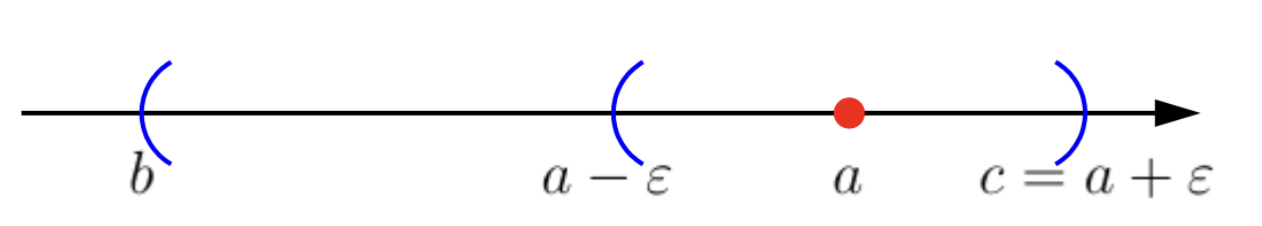
\includegraphics[scale=0.2]{Picture4.png}

\caption{  $b<a<c$ and $\varepsilon=c-a\leq a-b$.}\label{figure4}
\end{figure}
Next, we revisit the concept of denseness.
\begin{theorem}[label=23020409]{}
Let $S$ be a subset of real numbers. Then $S$ is dense in $\mathbb{R}$  if and only if every real number $x$ is the limit of a sequence in $S$.
\end{theorem}

Since we have proved that each of the set of rational numbers and the set of irrational numbers  is dense in the set of real numbers, we immediately obtain the following.
\begin{corollary}{}
Let $x$ be a real number.
\begin{enumerate}[1.]
\item
There is a sequence of rational numbers $\{p_n\}$ that converges to $x$.
\item There is a sequence of irrational numbers $\{q_n\}$ that converges to $x$.
\end{enumerate}
\end{corollary}


\begin{myproof}{\linkt Proof of Theorem \ref{23020409}}

First we assume that the set $S$ is dense in $\mathbb{R}$. Given a real number $x$, we want to show that there is a sequence in $S$ that converges to $x$. For each positive integer $n$, since $S$ is dense in $\mathbb{R}$, there is an element of $S$ in the open interval $(x-1/n, x)$. Choose one of these elements and denote it by $a_n$. Then $\{a_n\}$ is a sequence in $S$ satisfying
\[x-\frac{1}{n}<a_n<x\hspace{1cm}\text{for all}\;n\in\mathbb{Z}^+.\]
By squeeze theorem, the sequence $\{a_n\}$ converges to $x$.

 

Conversely, assume that every real number $x$ is the limit of a sequence in $S$. We want to show that $S$ is dense in $\mathbb{R}$. 
Let $(a,b)$ be an open interval. Take any point $x$ in the interval $(a,b)$.
By assumption, there is a sequence $\{c_n\}$ in $S$ which converges to $x$. By Lemma \ref{23020505}, the interval $(a,b)$ contains a point of $S$. Thus we have shown that every open interval $(a, b)$ contains a point of $S$. This proves that $S$ is dense in $\mathbb{R}$.
\end{myproof}

\begin{example}[label=23020501]{}
Let $x=\sqrt{2}$, and define the sequences $\{p_n\}$ and $\{q_n\}$ by
\[p_n=\frac{\lfloor 10^n\sqrt{2}\rfloor}{10^n}, \hspace{1cm} q_n=\sqrt{2}.\]
Here $\lfloor a\rfloor$ is the floor of $a$. By definition,
\[10^n\sqrt{2}-1<\lfloor 10^n\sqrt{2}\rfloor\leq 10^n\sqrt{2}.\]
Therefore,
\[\sqrt{2}-\frac{1}{10^n}<p_n\leq \sqrt{2}.\]
By squeeze theorem, 
$\{p_n\}$ converges to $\sqrt{2}$. Since $\lfloor 10^n\sqrt{2}\rfloor$ is an integer, $p_n$ is a rational number. Hence, $\{p_n\}$ is a sequence of rational numbers that converges to $x=\sqrt{2}$. Obviously, $\{q_n\}$ is a sequence of irrational numbers that converges to $x=\sqrt{2}$.
\end{example}
The number $p_n$ is the rational number obtained by truncating the decimal expansion of $\sqrt{2}$ to give a number with $n$ decimal places.
The first 7 terms of the sequence $\{p_n\}$ are
\[1.4, \;1.41, \;1.414, \;1.4142, \;1.41421,\; 1.414213,\; 1.4142135.\]

Now we introduce the concept  of closed sets.
\begin{definition}{Closed Set}
Let $S$ be a subset of $\mathbb{R}$. We say that $S$ is closed in $\mathbb{R}$ provided that if $\{a_n\}$ is a sequence of points in $S$ that converges to the limit $a$, the point $a$ is also in $S$. 
\end{definition}

\begin{example}{}
The three statements in Lemma \ref{23020406} imply that intervals of the form $(-\infty, a]$, $[a, \infty)$ and $[a,b]$ are closed subsets of $\mathbb{R}$. In particular, we call them closed intervals, and $[a,b]$ is a closed and bounded interval.
\end{example}


\begin{remark}{}
\begin{enumerate}[1.]
\item
By definition, $\mathbb{R}$ is closed in $\mathbb{R}$.
\item $\emptyset$ is closed in $\mathbb{R}$ because the statement that defines a closed set is a statement of the form $p\to q$, where $p$ is always false for an empty set. Hence, for an empty set, this statement $p\to q$ that defines a closed set is vacuously true.\end{enumerate}
\end{remark}

\begin{example}[label=23020502]{}
Is the interval $(0,2)$  closed in $\mathbb{R}$?
\end{example}
\begin{solution}{Solution}
The sequence $\{1/n\}$ is a sequence in the interval $(0, 2)$ that converges to the point $0$ that is not in $(0,2)$. Hence, the interval $(0,2)$ is not closed in $\mathbb{R}$.
\end{solution}

\begin{remark}{}
One can prove that if $S$ is an interval of the form $(a, b)$, or $(a, b]$, or $[a, b)$, or $(-\infty, a)$, or $(a, \infty)$, then $S$ is not closed in $\mathbb{R}$.
\end{remark}

\begin{example}{}
Is the set of rational numbers $\mathbb{Q}$ closed in $\mathbb{R}$? 
\end{example}
\begin{solution}{Solution}
We have seen in 
Example \ref{23020501} that there is a sequence in the set $\mathbb{Q}$ that converges to $\sqrt{2}$, which is not in $\mathbb{Q}$. Hence, $\mathbb{Q}$ is not closed in $\mathbb{R}$.
\end{solution}

The concept of closed sets is defined in terms of limits of sequences. This leads us to the concept of limit points.
\begin{definition}{Limit Points}
Let $S$ be a subset of real numbers. A point $x$ in $\mathbb{R}$ is called a limit point of the set $S$ if there is a sequence of points in $S\setminus \{x\}$ that converges to $x$.
\end{definition}
 
Notice that  $\{a_n\}$ is a sequence in $S\setminus\{x\}$ if and only if it is a sequence in $S$ with none of the terms $a_n$  equal to $x$. 
\begin{example}[label=23020503]{}
In the solution of Example \ref{23020502}, we have seen that the sequence $\{1/n\}$ in $(0,2)$  converges to the point $0$. Since none of the $a_n$ is 0,  0 is a limit point of the set $(0,2)$. 
\end{example}
\begin{highlight}{Limits and Limit Points}
Although the concepts of limits and limit points are closely related, one should not get confused. The limit of a convergent sequence $\{a_n\}$ is not necessarily the limit point of the set $\{a_n\,|\,n\in\mathbb{Z}^+\}$. For example, $c$ is the limit of the constant sequence $\{a_n\}$ with $a_n=c$ for all $n\in\mathbb{Z}^+$, but $c$ is not a limit point of the set $\{a_n\,|\,n\in\mathbb{Z}^+\}=\{c\}$.\end{highlight}

\begin{example}{}
Determine the set of limit  points of the set $(0,2)$.
\end{example}
\begin{solution}{Solution}
We claim that every point in $[0,2]$ is a limit point of the  set $(0,2)$. 

Example \ref{23020503} shows that 0 is a limit point of $(0,2)$. The sequence
$\{2-1/n\}$ is a sequence in $(0,2)$ that converges to 2. Hence, 2 is also a limit point of $(0,2)$.

For any $c\in (0,2)$, $c>0$. Let $m$ be a positive intger such that $1/m<c$. Then $\{c-1/(n+m)\}$ is  a sequence in $(0,2)$ that converges to $c$. Hence,  $c$ is a limit point of $(0,2)$.

This completes the proof that the set of limit points of $(0,2)$  is $[0,2]$.
\end{solution}

\begin{remark}{}
\begin{enumerate}[1.]
\item For intervals of the form $(a,b)$, $(a, b]$, $[a, b)$ or $[a,b]$, the set of limit points is $[a,b]$.
\item For intervals of the form $(-\infty, a)$ or $(-\infty, a]$, the set of limit points is $(-\infty, a]$.
\item For intervals of the form $(a, \infty)$ or $[a, \infty)$, the set of limit points is $[a, \infty)$.
\end{enumerate}

\end{remark}



\begin{example}[label=230322_1]{}
Show that the set $\mathbb{Z}$ does not have limit points.
\end{example}

\begin{solution}{Solution}

If $n$ is an integer, $x$ is contained in the open interval $(n-1,n+1)$ that does not contain any integer other than $n$ itself. Hence, there is no sequence in $\mathbb{Z}\setminus \{n\}$ that converges to $n$. Therefore, an integer $n$ is not a limit point of $\mathbb{Z}$.\bs

If $x$ is not an integer, it is contained in the interval $(\lfloor x\rfloor, \lceil x\rceil)$ that does not contain any integers. By Lemma \ref{23020505}, $x$ is not a limit of a sequence in $\mathbb{Z}$. Therefore, $x$ is not a limit point of $\mathbb{Z}$.
\end{solution}


\begin{definition}{Isolated Points}
Let $S$ be a subset of real numbers. We say that $x$ is an isolated point of $S$ if 
\begin{enumerate}[(a)]
\item $x$ is in $S$;
\item $x$ is not a limit point of $S$.
\end{enumerate}
\end{definition}

By definition, we have the following.
\begin{highlight}{Isolated Points vs Limit Points}
A point in a set $S$ is either a limit point or an isolated point of the set.
\end{highlight}

\begin{example}{}
By Example \ref{230322_1}, every point in the set of integers $\mathbb{Z}$ is an isolated point of the set.
\end{example}

The following is quite obvious from the definition of isolated points and Lemma \ref{23020505}.
\begin{theorem}[label=23020810]{}
Let $S$ be a subset of real numbers. A point $x$ in $S$ is an isolated  point if and only if there is a neighbourhood  $(a,b)$ of  $x$ that intersects the set $S$ only at the point $x$.
\end{theorem}

We have seen that a limit point of a set is not necessarily a point of that set. The following gives a characterization of closed sets in terms of limit points.
\begin{theorem}{}
Let $S$ be a subset of real numbers. The set $S$ is closed in $\mathbb{R}$ if and only if it contains all its limit points.

\end{theorem}
To prove a statement of the form $p\iff q$, we can prove $p\implies q$ and $\neg p \implies \neg q$.
\begin{myproof}{Proof}
Assume first $S$ is closed in $\mathbb{R}$. Let $x$ be a limit point of $S$. Then there is a sequence $\{a_n\}$ in $S\setminus\{x\}$ that converges to $x$. In particular, $\{a_n\}$ is a sequence in $S$ that converges to $x$. Since $S$ is closed in $\mathbb{R}$, $x$ is in $S$. This proves that $S$ contains all its limit points.


Now assume that $S$ is not closed in $\mathbb{R}$. Then there is a sequence $\{a_n\}$ in $S$ that converges to a point $x$, but $x$ is not in $S$. Since $x$ is not in $S$, none of the terms in the sequence $\{a_n\}$ is in $S$. Therefore, $x$ is a limit point of $S$. This shows that $S$ does not contain all its limit points.
\end{myproof}

\vp
\noindent
{\bf \large Exercises  \thesection}
\setcounter{myquestion}{1}

 \begin{question}{\themyquestion} 
 Show  that every real number is a limit point of the set of rational numbers.

\end{question}

\atc
 \begin{question}{\themyquestion} 
Let $S$ be the set
\[S=\left\{\left.\frac{1}{n}\,\right|\,n\in\mathbb{Z}^+\right\}\;\cup\;\{0\}.\]
\begin{enumerate}[(a)]
\item Find the set of limit points and the set of isolated points of $S$.
\item Is $S$ a closed set?
\end{enumerate}
\end{question}

\atc


 \begin{question}{\themyquestion} 
 Determine whether each of the following is a closed set.
\begin{enumerate}[(a)]\item $A=[2, 3]\;\cup\;[4, 7]$
\item $B=(-\infty, 2]\cup [3, 5]$
\item $C=\mathbb{R}\setminus (-1,1)$
\item $D=[1, 2)\cup [2, 4]$
\item $E=(1, 2)\cup (3, 4]$
\end{enumerate}
\end{question}

\vp
\section{The Monotone Convergence Theorem}\label{sec1.7}



Recall that a  sequence $\{a_n\}$ is monotone if it is increasing or it is decreasing. Obviously,  an increasing sequence is bounded below, and a decreasing sequence is  bounded above. However, a monotone sequence is not necessary convergent. A simple example is the sequence of natural numbers $\{n\}$. In the following, we give a characterization for a monotone sequence to be convergent. 
\begin{theorem}{The Monotone Convergence Theorem}
Let $\{a_n\}$ be a monotone sequence.
\begin{enumerate}[1.]
\item If $\{a_n\}$ is increasing, then $\{a_n\}$ is convergent if and only if it is bounded above. In this case, 
\[\lim_{n\rightarrow\infty}a_n=\sup \{a_n\}.\]
\item If $\{a_n\}$ is decreasing, then $\{a_n\}$ is convergent if and only if it is bounded below. In this case, 
\[\lim_{n\rightarrow\infty}a_n=\inf \{a_n\}.\]
\end{enumerate}
\end{theorem}
\begin{highlight}{Convergence Criteria for Monotone Sequences}
The monotone convergence theorem says that a montonone sequence is convergent if and only if it is bounded.
\end{highlight}
It is suffices to prove the case where $\{a_n\}$ is an increasing sequence. 
\begin{myproof}{Proof}
First suppose that $\{a_n\}$ is an increasing sequence that is convergent.  Then $\{a_n\}$ is bounded. So it is bounded above.

Conversely, suppose that $\{a_n\}$ is an increasing sequence that is bounded above. Then $a=\sup  \{a_n\}$ exists.  Now we use the same argument as in the proof of Lemma \ref{23020510}. Given $\varepsilon>0$, since $a-\varepsilon$ is less than $a$, it is not an upper bound of the set $S=\{a_n\,|\,n\in\mathbb{Z}^+\}$. Hence, there is a positive integer $N$ such that
\[a_N>a-\varepsilon.\]\bp
It follows that
\[a_n\geq a_N>a-\varepsilon\hspace{1cm}\text{for all}\;n\geq N.\]
Since $a$ is an upper bound of $S$, we also have $a_n\leq a$ for all $n$.  Thus,
\[|a_n-a|<\varepsilon\hspace{1cm}\text{for all}\;n\geq N.\]
This shows that the sequence $\{a_n\}$ converges to $a$.
\end{myproof}

The monotone convergence theorem is very useful because we can conclude the convergence of a sequence without apriori knowing  the limit of the sequence.  It is a consequence of the completeness axiom which asserts that any set that is bounded above has a supremum.  

\begin{example}[label=23020511]{}Let $a$ be a number in the interval $(0,1)$. Show that
\[\lim_{n\rightarrow\infty}a^n=0.\]

\end{example}

\begin{remark}{}

It follows from Theorem \ref{thm23020307} that for any $a$ in the interval $(-1,1)$, 
\[\lim_{n\rightarrow\infty}a^n=0.\]
\end{remark}

\begin{solution}{\linkt Solution to Example \ref{23020511}\linko}
Since $0<a<1$, for any positive integer $N$,
\[a^{n+1}=a^n\times a<a^n.\]
Hence, the sequence $\{a^n\}$ is decreasing.  On the other hand, $a^n>0$ for all $n\in\mathbb{Z}^+$. Hence, $\{a^n\}$ is a   decreasing sequence that is bounded below. By the monotone convergence theorem, $\{a^n\}$ converges to a number $\ell$. 
\bs
Since $\{a^{n+1}\}$ is a subsequence of $\{a^n\}$, it also converges to $\ell$.
Applying limit law to 
\[a^{n+1}=a\times a^n,\]
we have
\[\ell=\lim_{n\rightarrow\infty}a^{n+1}=a\lim_{n\rightarrow\infty}a^n=a\ell.\]
Since $a\neq 1$, we must have $\ell=0$.
\end{solution}

\begin{example}[label=23020512]{}
Define the sequence $\{a_n\}$ inductively by $a_1=1$ and for all $n\geq 1$,
\[a_{n+1}=\frac{2a_n+2}{a_n+2}.\]
Show that $\{a_{n}\}$ is convergent and find its limit.
\end{example}

\begin{solution}
{Solution} 
First notice that $a_n>0$ for all $n\in\mathbb{Z}^+$. 
When $n\geq 2$,
\[
a_{n+1}-a_n =\frac{2a_n+2}{a_n+2}-\frac{2a_{n-1}+2}{a_{n-1}+2}
 =\frac{2(a_n-a_{n-1})}{(a_n+2)(a_{n-1}+2)}.
\] Now, $a_2=4/3>a_1$. Hence, we deduce that $a_{n+1}-a_n>0$ for all $n\in\mathbb{Z}^+$.  In other words, $\{a_{n}\}$ is an increasing sequence.
 For all $n\geq 1$,
\[a_{n+1}=2-\frac{2}{a_n+2}<2.\]
Hence, $\{a_n\}$ is bounded above by 2.
Since $\{a_n\}$ is an increasing sequence that is bounded above, by monotone convergence theorem, it converges to a limit $u=\sup\{a_n\}$. 
Since $\{a_{n+1}\}$ is a subsequence of $\{a_n\}$,  it also converges to $u$. Apply the limit laws to \[a_{n+1}=\frac{2a_n+2}{a_n+2},\]we find that
\[u=\frac{2u+2}{u+2}.\]\bs
This implies that 
\[u^2=2.\]
Since $a_n>0$, we must have $u\geq 0$.  Hence, $u=\sqrt{2}$.

\end{solution}
Notice that Example \ref{23020512} is closely related to Example \ref{ex23020101}. The sequence $\{a_n\}$ defined in Example \ref{23020512}  is another sequence of rational numbers which converges to $\sqrt{2}$.


The next example is a classical one.

\begin{example}[label=23020507]{}
 

Show  that the limit
\[\lim_{n\rightarrow\infty} \left(1+\frac{1}{n}\right)^n\] exists. 
 
\end{example}



\begin{solution}{Solution}Let \[a_n=\left(1+\frac{1}{n}\right)^n.\]
  Given a positive integer $n$, notice that
\[\frac{ a_{n+1}}{a_n}=\frac{n+2}{n+1}\times \left(\frac{(n+2)n}{(n+1)^2}\right)^n.\]
By Bernoulli's inequality (see Question \ref{Q23020501}), 
\begin{align*}
 \left(\frac{(n+2)n}{(n+1)^2}\right)^n=\left(1-\frac{1}{(n+1)^2}\right)^n\geq 1-\frac{n}{(n+1)^2}=\frac{n^2+n+1}{(n+1)^2}.
\end{align*}
It follows that
\begin{align*}
\frac{a_{n+1}}{a_n}\geq \frac{(n+2)(n^2+n+1)}{(n+1)^3}=\frac{n^3+3n^2+3n+2}{n^3+3n^2+3n+1}>1.
\end{align*}
This shows that 
\[a_{n+1}>a_n\hspace{1cm}\text{for all}\;n\in\mathbb{Z}^+.\]\bs
Hence, $\{a_n\}$ is monotonically increasing.
 Using binomial expansion, we have
\[a_n=\sum_{k=0}^{n}\binom{n}{k}\frac{1}{n^k}.\]
For $k\geq 1$, Question \ref{Q23020502} shows that
\[\binom{n}{k}\frac{1}{n^k}=\frac{1}{k!}\frac{n(n-1)\cdots (n-k+1)}{n^k}\leq \frac{1}{k\,!}\leq \frac{1}{2^{k-1}}.\]
Therefore,
\[a_n\leq 1+1+\frac{1}{2}+\cdots+\frac{1}{2^{n-1}}=3-\frac{1}{2^{n-1}}\leq 3.\]
This proves that $\{a_n\}$ is bounded above by 3.
  Since $\{a_n\}$ is an increasing sequence that is bounded above, the monotone convergence theorem asserts that the limit
\[\lim_{n\rightarrow\infty}a_n=\lim_{n\rightarrow\infty} \left(1+\frac{1}{n}\right)^n\] exists. 
 
\end{solution}

\begin{highlight}{The Number $\pmb{e}$}
The number $e$ is defined as  
\[e=\lim_{n\rightarrow\infty} \left(1+\frac{1}{n}\right)^n.\] Correct to 15 decimal places, its numerical value is
\[e=2.718281828459046\]

One can show that the sequence $\{b_n\}_{n=0}^{\infty}$ defined by $b_0=1$, 
\[b_n=b_{n-1}+\frac{1}{n!}\hspace{1cm}\text{for all}\; n\geq 1,\]
also converges to $e$. In series notation, 
\[e=1+\frac{1}{1!}+\frac{1}{2!}+\frac{1}{3!}+\cdots+\frac{1}{n!}+\cdots.\]
\end{highlight}


\vp
\noindent
{\bf \large Exercises  \thesection}
\setcounter{myquestion}{1}


 \begin{question}{\themyquestion} 
Given that the sequence $\{a_n\}$ is defined by $a_1=2$, and for all $n\geq 1$,
\[a_{n+1}=\frac{3a_n+1}{a_n+2}.\]
Show that $\{a_n\}$ is convergent and find its limit.
\end{question}
\atc

 \begin{question}{\themyquestion} 
 For $n\geq 1$, let
\[a_n=\left(1+\frac{1}{n}\right)^n.\]
Define the sequence $\{b_n\}_{n=0}^{\infty}$ by $b_0=1$, and for all $n\geq 1$,
\[b_n=b_{n-1}+\frac{1}{n!}.\]

\begin{enumerate}[(a)]
\item Show that the sequence $\{b_n\}$ is convergent.
\item For a positive integer $n$, use the binomial expansion of $a_n$ to show that 
$a_n\leq b_n$ and 
\[b_n-a_n\leq\frac{3}{2n}.\]
\item Conclude that the sequence $\{b_n\}$ converges to $e$.
\end{enumerate}
 
\end{question}
\vp
\section{Sequential Compactness}\label{sec1.8}

Let us first look at an example.
 \begin{example}{}
 Let $\{a_n\}$ be the sequence defined by
 \[a_n=(-1)^{n-1}\frac{n}{n+1}.\]
 Obviously,
 \[|a_n|=\frac{n}{n+1}\leq 1.\] 
 Hence, the sequence $\{a_n\}$ is bounded. 
 Now,
 \[a_{2n-1}=\frac{2n-1}{2n},\hspace{1cm}a_{2n}=-\frac{2n}{2n+1}.\]
 The subsequence $\{a_{2n-1}\}$ converges to 1, whereas the subsequence $\{a_{2n}\}$ converges to $-1$. Since there are two subsequences that converge to two different limits,
 the sequence $\{a_n\}$ is not convergent.
 
 \end{example}
In this example, we find that although the sequence $\{a_n\}$ is not convergent, it has convergent subsequences.
 In this section, we are going to  prove that every bounded sequence has a convergent subsequence.
By monotone convergence theorem, it is sufficient to prove that every sequence has a monotone subsequence. It can be achieved via a concept called peak index.
 
 \begin{definition}{Peak Index}
 Let $\{a_n\}$ be a sequence of real numbers. A positive integer $m$ is called a {\bf peak index} of the sequence if 
 \[a_m\geq a_n\hspace{1cm}\text{for all}\;n\geq m.\]In other words,   there is no term after the $m^{\text{th}}$ term that is larger than $a_m$.
 \end{definition}
 
 If $\{a_n\}$ is a decreasing sequence, every positive integer is a peak index of the sequence. If $\{a_n\}$ is an increasing sequence, $m$ is a peak index if and only if $a_n=a_m$ for all $n\geq m$, which means $\{a_n\}$ is a constant from the $m^{\text{th}}$ term on. We can use the concept of peak indices to prove the following.
 
 \begin{theorem}{}
 Every sequence has a monotone subsequence.
 \end{theorem}
 \begin{myproof}{Proof}
 Given a sequence $\{a_n\}$, let $S$ be the set of its peak indices. It is a subset of positive integers.  We discuss the cases where $S$ is infinite and $S$ is finite.
 
 \textbf{Case 1:} $S$ is infinite.\\
Let
 $n_1, n_2, n_3, \ldots$ be the elements of $S$  arranged in increasing order, namely,
 \[n_1<n_2<n_3<\cdots.\] This is a subsequence of $\{n\}$. For any positive integer $k$, since $n_{k+1}>n_k$ and $n_k$ is a peak index, we have
 \[a_{n_{k+1}}\leq a_{n_k}.\]
 This shows that $\{a_{n_k}\}$ is a decreasing subsequence of $\{a_n\}$.
 
 \textbf{Case 2:} $S$ is finite.\\If $S$ is an empty set, let $n_1=1$. If $S$ is not empty,   it has a largest element $n_{\max}$. Let $n_1=n_{\max}+1$. Then for any integer $n$ such that $n\geq n_1$, $n$ is not a peak index of the sequence. Since  $n_1$ is not a peak index, there is an $n_2>n_1$ such that
$a_{n_2}>a_{n_1}$.
 Suppose that we have chosen the positive integers $n_1, n_2, \ldots, n_k$ such that $n_1<n_2<\cdots<n_k$ and
 \[a_{n_1}<a_{n_2}<\cdots<a_{n_k}.\]

 Now $n_k$ is   not a peak index implies that there is a positive integer $n_{k+1}$ larger than $n_k$ such that
 \[a_{n_{k+1}}>a_{n_{k}}.\] 
 This procedure constructs the increasing subsequence $\{a_{n_k}\}$ inductively.
 
 In both cases, we have shown that $\{a_n\}$ has a monotone subsequence.
 \end{myproof}
 
 Obviously, a subsequence of a bounded sequence is bounded. It follows from the monotone convergence theorem the following important assertion.
 \begin{theorem}{Bolzano-Weierstrass Theorem}
 Every bounded sequence has a convergent subsequence.
 \end{theorem}
 


Now we want to introduce a concept called Cauchy sequence, which is closely related to completeness axiom.
\begin{definition}{Cauchy Sequence}
A sequence $\{a_n\}$ is called a {\bf Cauchy sequence} provided that for any $\varepsilon>0$, the is a positive integer $N$ such that for all $m\geq n\geq N$,
\[|a_m-a_n|<\varepsilon.\]

\end{definition}
\begin{example}{}
For the sequence $\{a_n\}$ with $a_n=\di\frac{n+1}{n}$,  it is easy to check that it is a Cauchy sequence. Notice that if $m\geq n$,
\[|a_m-a_n|=\left|\frac{1}{n}-\frac{1}{m}\right|=\frac{1}{n}-\frac{1}{m}<\frac{1}{n}.\]
Given $\varepsilon>0$, the Archimedean property says that there is a positive integer $N$ such that $1/N<\varepsilon$. Hence, if $m\geq n\geq N$,
\[|a_m-a_n|<\frac{1}{n}\leq\frac{1}{N}<\varepsilon.\]
\end{example}

There is a similarity between the definition of a Cauchy sequence  and the definition of convergence of a sequence.  We can show that a linear combination of Cauchy sequences is a Cauchy sequence, and a product of Cauchy sequences is a Cauchy sequence. For the quotient, some care need to be taken.   We leave it to the students to formulate the precise statement.




In the definition of a Cauchy sequence, we do not need to know whether the sequence is convergent, or what is the limit of the sequence if it is convergent.
Nevertheless,   a convergent sequence is a Cauchy sequence.

\begin{theorem}[label=23020602]{}
If a sequence $\{a_n\}$ is convergent, then it is a Cauchy sequence.
\end{theorem}
\begin{myproof}{Proof}
Let $a$ be the limit of the convergent sequence $\{a_n\}$. Given $\varepsilon>0$, there is a positive integer $N$ such that for all $n\geq N$,
\[ |a_n-a|<\frac{\varepsilon}{2}.\]
It follows from triangle inequality that if $m\geq n\geq N$,
\[|a_m-a_n|\leq |a_m-a|+|a_n-a|<\frac{\varepsilon}{2}+\frac{\varepsilon}{2}=\varepsilon.\]
Hence, $\{a_n\}$ is a Cauchy sequence.
\end{myproof}

The converse is also true \emph{in the set of real numbers}. It is proved using the fact that every bounded sequence has a convergent subsequence.

\begin{theorem}[label=23020603]{Cauchy Criterion for Convergent Sequennce}
If $\{a_n\}$ is a Cauchy sequence of real numbers, then it converges to a real number.
\end{theorem}
\begin{myproof}
{Proof}First we prove that   $\{a_n\}$ is a Cauchy sequence implies that it is bounded. The proof is almost identical to the proof that a convergent sequence is bounded.
Take $\varepsilon=1$. There is  a positive integer $N_0$ such that for all $m\geq n\geq N_0$, 
\[|a_m-a_n|<1.\]
This implies that 
\[|a_m|\leq |a_{N_0}|+1\hspace{1cm}\text{for all}\;m\geq {N_0}.\]\bp
Let
\[M=\max\{|a_1|, \ldots, |a_{N_0-1}|, |a_{N_0}|+1.\}\] Then $|a_n|\leq M$ for all $n\in\mathbb{Z}^+$, proving that it is bounded.
Since $\{a_n\}$ is a bounded sequence, it has a convergent subsequence $\{a_{n_k}\}$ which converges to a limit $a$. We want to prove that the sequence $\{a_n\}$ also converges to $a$.
Given $\varepsilon>0$, there is a positive integer $N$ such that for all $m\geq n\geq N$,
\[|a_{m}-a_n|<\frac{\varepsilon}{2}.\]
There is a positive integer $K$ such that for all $k\geq K$,
\[|a_{n_k}-a|<\frac{\varepsilon}{2}.\]
 Now let $n$ be an integer such that $n\geq N$. Since $\{n_k\}$ is a subsequence of $\{n\}$, there is an integer $k$ such that $k\geq K$ and $n_k\geq n$. Then
\[|a_n-a|\leq |a_{n_k}-a_n|+|a_{n_k}-a|<\frac{\varepsilon}{2}+\frac{\varepsilon}{2}=\varepsilon.\]

 This proves that for all $n\geq N$,
\[|a_n-a|<\varepsilon.\] Hence, the sequence $\{a_n\}$ indeed converges to $a$.
\end{myproof}
 Theorem \ref{23020603} is proved using the fact that every bounded sequence has a convergent subsequence. The latter is a consequence of the monotone convergence theorem, whose validity relies on the completeness axiom for real numbers.
 Hence, the fact that every Cauchy sequence of real numbers is convergent is a consequence of the completeness axiom.
 
   If we consider the set of rational numbers, the assertion is not true. For example, we have shown that there is a sequence of rational numbers $\{a_n\}$ that converges to $\sqrt{2}$. Therefore, the sequence $\{a_n\}$ is a Cauchy sequence that does not converge in the set of rational numbers. 

The following combines the results of Theorem \ref{23020602} and Theorem \ref{23020603}.
\begin{highlight}{Cauchy Criterion for Convergent Sequennce}
A sequence of real numbers $\{a_n\}$ is convergent if and only if it is a Cauchy sequence.
\end{highlight}

As the monotone convergence theorem, the Cauchy criterion can be used to conclude the convergence of a sequence without apriori knowing the limit of the sequence. It has wide applications as we are going to see in latter chapters. 
\begin{example}
{}For a positive integer $n$, let
\[s_n=1+\frac{1}{2}+\cdots+\frac{1}{n}.\]
Show that the sequence $\{s_n\}$ is divergent.

\end{example}
\begin{solution}{Solution}
We prove that $\{s_n\}$ is not a Cauchy sequence, by showing that for $\varepsilon=1/2$, for any positive integer $N$, there are integers $m$ and $n$ with $m\geq n\geq N$ such that 
\[|s_m-s_n|\geq \frac{1}{2}.\]
For a given positive integer $N$, let $n=N$ and $m=2N$. Then $m\geq n\geq N$ and $m-n=N$.   Notice that
\begin{align*}s_m-s_n&=\frac{1}{N+1}+\frac{1}{N+2}+\cdots+\frac{1}{2N}\\& \geq \underbrace{\frac{1}{2N}+\frac{1}{2N}+\cdots+\frac{1}{2N}}_{m-n=N\;\text{terms}}\\&=\frac{1}{2}.\end{align*}This shows that $\{s_n\}$ is not a Cauchy sequence. Hence, it is not convergent.
\end{solution}

We have studied the convergence   of sequences, and the interplay between sequences and sets.
Now we define another property of sets called sequential compactness.
 \begin{definition}{Sequential Compactness}
 Let $S$ be a subset of real numbers. We say that $S$ is {\bf sequentially compact}  provided that   every sequence in $S$ has a subsequence that converges to a point in $S$.
 \end{definition}
 Using logic, we find that a set $S$ is not sequentially compact if there is a sequence in $S$ that do not have a convergent subsequence with limit in $S$.
 
 From the theories that we have developed in this chapter, it is not difficult to prove the following.
 \begin{theorem}[label=23020604]{}
 If $S$ is a closed and bounded subset of real numbers, then it is sequentially compact.
 \end{theorem}
 \begin{myproof}{Proof}
 Let $S$ be a subset of $\mathbb{R}$ that is closed and bounded.  Given a sequence $\{a_n\}$ in $S$, since $S$ is bounded,   the sequence $\{a_n\}$ is bounded. Therefore, there is a subsequence $\{a_{n_k}\}$ that converges to a number $a$. Since $\{a_{n_k}\}$ is a sequence in the  set $S$ that converges to  $a$, and $S$ is closed,  the limit $a$ must be in $S$. In other words, we have shown that the sequence $\{a_n\}$ in $S$ has a subsequence $\{a_{n_k}\}$ that converges to  a point $a$ that is in $S$. This proves that $S$ is sequentially compact.
 \end{myproof}
 
 \begin{example}{}
 Since an interval of the form $[a,b]$ is closed and bounded, it is sequentially compact.
 \end{example}
 
 The converse to Theorem \ref{23020604} is also true.
 \begin{theorem}[label=23020707]{}
Let $S$ be a subset of $\mathbb{R}$. If $S$ is sequentially compact, then it is closed and bounded.
 \end{theorem}
 This is a statement of the form $p\to q\wedge r$. It is equivalent to $(p\to q)\wedge (p\to r)$, which in turn is equivalent to $(\neg q\to \neg p)\wedge (\neg r\to \neg p)$. Hence, we will prove the following two statements: if $S$ is not closed, it is not sequentially compact; and if $S$ is not bounded, it is not sequentially compact.
 \begin{myproof}{Proof}
 First, we prove that if $S$ is not closed, it is not sequentially compact. If $S$ is not closed, there is a sequence $\{a_n\}$ in $S$ which converges to a point $a$ but $a$ is not in $S$. For this sequence, every subsequence is convergent with limit $a$. Hence, this sequence does not have a convergent subsequence with limit in $S$. This proves that $S$ is not sequentially compact.
 
 Next, we prove that if $S$ is not bounded, it is not sequentially compact. If $S$ is not bounded, for each integer $n$, there is a point $a_n$ in $S$ such that
 \[|a_n|\geq n.\]Consider the sequence $\{a_n\}$. If $\{a_{n_k}\}$ is a subsequence of $\{a_n\}$,
 \[|a_{n_k}|\geq n_k.\] Hence, the sequence
  $\{a_{n_k}\}$ is not bounded, and thus it is not convergent. This shows that the sequence $\{a_n\}$ does not have any convergent subsequence. Therefore, $S$ is not sequentially compact.
 
  
 \end{myproof}
 Combining Theorem \ref{23020604} and Theorem \ref{23020707}, we have the following.
 \begin{highlight}{Characterization of Sequentially Compact Sets}
 A subset of real numbers is sequentially compact if and only if it is closed and bounded.
 \end{highlight}
 
 Notice that the only type of intervals that is both closed and bounded is the type $[a, b]$. Hence, this is the only type of  intervals that are sequentially compact.
 \begin{example}{}
 Determine whether each of the following sets is sequentially compact.
 \begin{enumerate} [(a)]
  \item $\mathbb{Z}$
  \item 
 $A=[2, 5]\setminus\{3\}$

 
 \item  $B=(0, 6]\cap [4, 7]$.
 \end{enumerate}
 \end{example}
 \begin{solution}{Solution}
  \begin{enumerate}[(a)]
  \item The set $\mathbb{Z}$ is not bounded. Hence, it is not  sequentially compact.
  \item  $3$ is a limit point of the set $A$ but it is not in $A$. Hence, $A$ is not closed, and so it is not  sequentially compact. 
  \item  $B=[4, 6]$ is closed and bounded. Hence, $B$ is sequentially compact.
  \end{enumerate}
 \end{solution}
 
It might be wondered why there is a need to introduce the concept of sequential compactness if it is equivalent to closed and bounded.    We will see that for a subset of real numbers that is closed and bounded, every sequence in that set has a subsequence that converges to a point in that set  is   a very important characteristic. By introducing the concept of sequential compactness, we can avoid repeatedly proving this property for a set that is closed and bounded.

The next theorem gives an important feature of a sequentially compact set.
\begin{theorem}[label=23020908]{}Let $S$ be a subset of real numbers. If $S$ is closed and bounded, then it has a maximum and a minimum. Equivalently, if $S$ is sequentially compact, then it has a maximum and a minimum.
\end{theorem}
\begin{myproof}{Proof}
 Since $S$ is bounded, $S$ has a least upper bound $u$ and a greatest lower bound $\ell$. By Lemma \ref{23020510}, there are sequences $\{u_n\}$ and $\{\ell_n\}$ in $S$ that converge to $u$ and $\ell$ respectively. Since $S$ is closed, $u$ and $\ell$ are in $S$. Since $u=\sup S$ is in $S$, $S$ has a maximum. Since $\ell=\inf S$ is in $S$, $S$ has a minimum.
\end{myproof}
\vp
\noindent
{\bf \large Exercises  \thesection}
\setcounter{myquestion}{1}
 \begin{question}{\themyquestion} 
Given that the sequence $\{a_n\}$ is defined by
\[a_n=1+\frac{1}{3}+\ldots+\frac{1}{2n-1}.\]
Show that $\{a_n\}$ is not a Cauchy sequence. Then conclude that the sequence $\{a_n\}$ is divergent.
\end{question}
 
 \atc

 \begin{question}{\themyquestion} 
Determine whether each of the following sequence is a Cauchy sequence.
\begin{enumerate}[(a)]
\item The sequence $\{a_n\}$ with $a_n=\di \frac{n+(-1)^n}{n-(-1)^n}$
\item The sequence $\{b_n\}$ with $b_n=\di \frac{1+  n}{1-(-1)^n n}$

\end{enumerate}
\end{question}
\atc
 \begin{question}{\themyquestion} 
 Determine whether each of the following sets is sequentially compact.
 \begin{enumerate} [(a)]
  \item $A=\{1, 2, \cdots, 100\}$
  \item 
 $B=[4, 7]\cap (6, 8]$

 
 
 \end{enumerate}
\end{question}
 
\atc
 \begin{question}{\themyquestion} 
Show that the union of two sequentially compact sets is sequentially compact. 
\end{question}
